\documentclass[11pt,a4paper]{article}
\usepackage[utf8]{inputenc}
\usepackage[T1]{fontenc}
\usepackage{lmodern}
\usepackage{textcomp}
\usepackage{amsmath,amssymb}
\usepackage{graphicx}
\usepackage{booktabs}
\usepackage{longtable}
\usepackage{array}
\usepackage{listings}
\usepackage{xcolor}
\usepackage[margin=1in]{geometry}
\usepackage{float}
\usepackage[hidelinks,breaklinks]{hyperref}
\usepackage{microtype}
\setlength{\parskip}{4pt}
\lstset{basicstyle=\ttfamily\scriptsize,breaklines=true,breakatwhitespace=false,
  postbreak=\mbox{\textcolor{gray}{$\hookrightarrow$}\space},frame=single,
  framerule=0.3pt,rulecolor=\color{gray!60},columns=fullflexible,keepspaces=true,
  showstringspaces=false,numbers=none,xleftmargin=4pt,xrightmargin=4pt,
  literate={\_}{{\_}}1}
\graphicspath{{figures/}}
\providecommand{\tightlist}{}
\title{Supplementary material: The Thermal Pure Higgsino near 1.1 TeV versus Planck 2018, LZ 2024 and XENONnT: A Literature-Based Assessment}
\author{HEP-Genesis-Agent session record \\ \small Project: ramp-research-higgsino-dd}
\date{2026-10-16}
\begin{document}
\maketitle
\noindent\textit{\small Supplementary material, generated mechanically from the session record: it lists exactly what ran, in order, without interpretation.}
\vspace{1em}



\appendix
\section{Implementation details}
\label{app:impl}
This appendix is generated mechanically from the session record; it lists exactly what ran, in order, without interpretation.
\subsection{Session}
\begin{itemize}
  \item Source: cli client; conversation \texttt{9e56c682}
  \item Started: 2026-10-16 11:03:59; report generated: 2026-10-16 11:14:04
  \item Project: ramp-research-higgsino-dd (\texttt{/\allowbreak{}Users/\allowbreak{}nramachandra/\allowbreak{}hep-genesis-testing/\allowbreak{}projects/\allowbreak{}ramp-research-higgsino-dd})
  \item Compute execution site(s) selected in the session: local
  \item 2 user turn(s), 103 tool call(s) (0 returned errors), 6 figure(s), 8 data file(s)
\end{itemize}
\subsection{Models}
\begin{longtable}{@{}p{0.16\textwidth}p{0.34\textwidth}p{0.44\textwidth}@{}}
\toprule Stage & Model & Endpoint \\ \midrule \endhead
quick & \texttt{claude-opus-5-5} & \texttt{https:\allowbreak{}/\allowbreak{}/\allowbreak{}mag.genesis.americansciencecloud.org/\allowbreak{}v1} \\
report & \texttt{claude-opus-5-5} & \texttt{https:\allowbreak{}/\allowbreak{}/\allowbreak{}mag.genesis.americansciencecloud.org/\allowbreak{}v1} \\
coder & \texttt{claude-opus-5-5} & \texttt{https:\allowbreak{}/\allowbreak{}/\allowbreak{}mag.genesis.americansciencecloud.org/\allowbreak{}v1} \\
\bottomrule\end{longtable}
\subsection{MCP servers}
\begin{longtable}{@{}p{0.22\textwidth}p{0.12\textwidth}p{0.6\textwidth}@{}}
\toprule Server & Transport & Location \\ \midrule \endhead
hep-research-aid & stdio & \texttt{python -m hep\_\allowbreak{}genesis.domain.mcp\_\allowbreak{}server} \\
alcf-tools & stdio & \texttt{python -m hep\_\allowbreak{}genesis.iri.alcf.mcp\_\allowbreak{}server} \\
nersc-tools & stdio & \texttt{python -m hep\_\allowbreak{}genesis.iri.nersc.mcp\_\allowbreak{}server} \\
\bottomrule\end{longtable}
\subsection{Tool-call log}
Chronological; arguments and results are truncated for space (the full record is in the project's \texttt{provenance/} folder).
\begin{longtable}{@{}p{0.04\textwidth}p{0.22\textwidth}p{0.36\textwidth}p{0.32\textwidth}@{}}
\toprule \# & Tool & Arguments & Outcome \\ \midrule \endhead
1 & \texttt{hep-research-aid}\newline\texttt{list\_\allowbreak{}agent\_\allowbreak{}files} & \texttt{\{\}\allowbreak{}} & \texttt{[]\allowbreak{}} \\
2 & \texttt{hep-research-aid}\newline\texttt{list\_\allowbreak{}input\_\allowbreak{}files} & \texttt{\{\}\allowbreak{}} & \texttt{\{   ''status'':\allowbreak{} ''success'',\allowbreak{}   ''files'':\allowbreak{} []\allowbreak{},\allowbreak{}   ''usage'':\allowbreak{} ''Pass any of these filenames to load\_\allowbreak{}table\_\allowbreak{}data()\allowbreak{}.'' \}\allowbreak{}} \\
3 & \texttt{hep-research-aid}\newline\texttt{list\_\allowbreak{}datasets} & \texttt{\{\}\allowbreak{}} & \texttt{\{'count':\allowbreak{} 0,\allowbreak{} 'datasets':\allowbreak{} []\allowbreak{}\}\allowbreak{}} \\
4 & \texttt{hep-research-aid}\newline\texttt{list\_\allowbreak{}files} & \texttt{\{\}\allowbreak{}} & \texttt{Files in .:\allowbreak{}   - .git   - .gitignore   - ISSUES.md   - SCOPE.md   - docs   - downloads   - logs   - projects   - reports   - research-results   - runs   - scripts   - venvs   - workspace} \\
5 & \texttt{hep-research-aid}\newline\texttt{get\_\allowbreak{}dispatch} & \texttt{\{\}\allowbreak{}} & \texttt{Dispatch:\allowbreak{} local execution.} \\
6 & \texttt{local}\newline\texttt{search\_\allowbreak{}arxiv\_\allowbreak{}abstracts} & \texttt{\{''query'':\allowbreak{} ''higgsino dark matter thermal relic 1.1 TeV direct detection'',\allowbreak{} ''max\_\allowbreak{}results'':\allowbreak{} 8\}\allowbreak{}} & \texttt{[2302.02905v2]\allowbreak{} Third family quasi-Yukawa unification:\allowbreak{} Higgsino dark matter,\allowbreak{} NLSP gluino and all that Abstract:\allowbreak{} We explore the implications of third family (\$t-b-$\tau$\$)\allowbreak{} quasi-Yukawa unification (QYU)\allowbreak{} for \ldots{}\allowbreak{}} \\
7 & \texttt{local}\newline\texttt{search\_\allowbreak{}arxiv\_\allowbreak{}abstracts} & \texttt{\{''query'':\allowbreak{} ''pure higgsino Sommerfeld enhancement relic abundance mass'',\allowbreak{} ''max\_\allowbreak{}results'':\allowbreak{} 5\}\allowbreak{}} & \texttt{[1008.2905v2]\allowbreak{} Thermal abundance of non-relativistic relics with Sommerfeld enhancement Abstract:\allowbreak{} We propose an analytic treatment for computing the relic abundances of non-relativistic particles whose\ldots{}\allowbreak{}} \\
8 & \texttt{local}\newline\texttt{search\_\allowbreak{}arxiv\_\allowbreak{}abstracts} & \texttt{\{''query'':\allowbreak{} ''higgsino inelastic dark matter mass splitting electroweak loop scattering'',\allowbreak{} ''max\_\allowbreak{}results'':\allowbreak{} 6\}\allowbreak{}} & \texttt{[0811.4682v1]\allowbreak{} Precision Electroweak Measurements and Constraints on the Standard Model Abstract:\allowbreak{}   This note presents constraints on Standard Model parameters using published and preliminary precision\ldots{}\allowbreak{}} \\
9 & \texttt{local}\newline\texttt{search\_\allowbreak{}arxiv\_\allowbreak{}abstracts} & \texttt{\{''query'':\allowbreak{} ''LZ 2024 WIMP search results spin-independent limits'',\allowbreak{} ''max\_\allowbreak{}results'':\allowbreak{} 4\}\allowbreak{}} & \texttt{[1509.02910v2]\allowbreak{} LUX-ZEPLIN (LZ)\allowbreak{} Conceptual Design Report Abstract:\allowbreak{} The design and performance of the LUX-ZEPLIN (LZ)\allowbreak{} detector is described as of March 2015 in this Conceptual Design Report. LZ is a sec\ldots{}\allowbreak{}} \\
10 & \texttt{hep-research-aid}\newline\texttt{search\_\allowbreak{}arxiv} & \texttt{\{''query'':\allowbreak{} ''pure higgsino dark matter spin-independent cross section two-loop electroweak direct detection'',\allowbreak{} ''max\_\allowbreak{}results'':\allowbreak{} 6\}\allowbreak{}} & \texttt{Found 6 papers matching query:\allowbreak{} 'pure higgsino dark matter spin-independent cross section two-loop electroweak direct detection' (source:\allowbreak{} arXiv API)\allowbreak{}  Paper 1:\allowbreak{} arXiv ID:\allowbreak{} 1901.09751v3 Title:\allowbreak{} Pseudo Nambu\ldots{}\allowbreak{}} \\
11 & \texttt{hep-research-aid}\newline\texttt{search\_\allowbreak{}arxiv} & \texttt{\{''query'':\allowbreak{} ''LZ dark matter search results 4.2 tonne-year exposure'',\allowbreak{} ''max\_\allowbreak{}results'':\allowbreak{} 4\}\allowbreak{}} & \texttt{Found 4 papers matching query:\allowbreak{} 'LZ dark matter search results 4.2 tonne-year exposure' (source:\allowbreak{} arXiv API)\allowbreak{}  Paper 1:\allowbreak{} arXiv ID:\allowbreak{} 2410.17036v3 Title:\allowbreak{} Dark Matter Search Results from 4.2 Tonne-Years of Ex\ldots{}\allowbreak{}} \\
12 & \texttt{hep-research-aid}\newline\texttt{search\_\allowbreak{}arxiv} & \texttt{\{''query'':\allowbreak{} ''XENONnT WIMP search first results nuclear recoil'',\allowbreak{} ''max\_\allowbreak{}results'':\allowbreak{} 4\}\allowbreak{}} & \texttt{Found 4 papers matching query:\allowbreak{} 'XENONnT WIMP search first results nuclear recoil' (source:\allowbreak{} arXiv API)\allowbreak{}  Paper 1:\allowbreak{} arXiv ID:\allowbreak{} 0809.3137v1 Title:\allowbreak{} The Frontiers of Nuclear Science,\allowbreak{} A Long Range Plan Authors\ldots{}\allowbreak{}} \\
13 & \texttt{hep-research-aid}\newline\texttt{search\_\allowbreak{}arxiv} & \texttt{\{''query'':\allowbreak{} ''higgsino dark matter neutrino floor next generation xenon detectors reach'',\allowbreak{} ''max\_\allowbreak{}results'':\allowbreak{} 6\}\allowbreak{}} & \texttt{Found 6 papers matching query:\allowbreak{} 'higgsino dark matter neutrino floor next generation xenon detectors reach' (source:\allowbreak{} arXiv API)\allowbreak{}  Paper 1:\allowbreak{} arXiv ID:\allowbreak{} 1211.7222v1 Title:\allowbreak{} Direct dark matter detection:\allowbreak{} the \ldots{}\allowbreak{}} \\
14 & \texttt{local}\newline\texttt{get\_\allowbreak{}arxiv\_\allowbreak{}metadata} & \texttt{\{''arxiv\_\allowbreak{}id'':\allowbreak{} ''2609.09830''\}\allowbreak{}} & \texttt{arXiv ID:\allowbreak{} 2609.09830 Title:\allowbreak{} Radiative Corrections to the Direct Detection of Inelastic Scattering of Higgsino-like Neutralino Dark Matter Authors:\allowbreak{} Arindam Chatterjee,\allowbreak{} Debottam Das,\allowbreak{} Syed Adil Pasha,\allowbreak{} Al\ldots{}\allowbreak{}} \\
15 & \texttt{local}\newline\texttt{search\_\allowbreak{}arxiv\_\allowbreak{}abstracts} & \texttt{\{''max\_\allowbreak{}results'':\allowbreak{} 5,\allowbreak{} ''query'':\allowbreak{} ''Hisano direct detection electroweak-interacting dark matter wino higgsino gluon contribution''\}\allowbreak{}} & \texttt{[1004.4090v1]\allowbreak{} A complete calculation for direct detection of Wino dark matter Abstract:\allowbreak{} In the anomaly-mediated supersymmetry (SUSY)\allowbreak{} breaking scenario,\allowbreak{} neutral gaugino of SU(2)\allowbreak{}\_\allowbreak{}L multiplet,\allowbreak{} Wino,\allowbreak{} can \ldots{}\allowbreak{}} \\
16 & \texttt{local}\newline\texttt{search\_\allowbreak{}arxiv\_\allowbreak{}abstracts} & \texttt{\{''max\_\allowbreak{}results'':\allowbreak{} 5,\allowbreak{} ''query'':\allowbreak{} ''XENONnT WIMP dark matter search combined science runs 2025''\}\allowbreak{}} & \texttt{[1211.0310v1]\allowbreak{} Large Synoptic Survey Telescope:\allowbreak{} Dark Energy Science Collaboration Abstract:\allowbreak{} This white paper describes the LSST Dark Energy Science Collaboration (DESC)\allowbreak{},\allowbreak{} whose goal is the study of dark\ldots{}\allowbreak{}} \\
17 & \texttt{local}\newline\texttt{search\_\allowbreak{}arxiv\_\allowbreak{}abstracts} & \texttt{\{''max\_\allowbreak{}results'':\allowbreak{} 4,\allowbreak{} ''query'':\allowbreak{} ''Planck 2018 results cosmological parameters''\}\allowbreak{}} & \texttt{[0604069v1]\allowbreak{} The Scientific Programme of Planck Abstract:\allowbreak{}   For 40 years,\allowbreak{} the cosmic microwave background (CMB)\allowbreak{} has been the most important source of information about the geometry and contents of the \ldots{}\allowbreak{}} \\
18 & \texttt{hep-research-aid}\newline\texttt{list\_\allowbreak{}input\_\allowbreak{}files} & \texttt{\{\}\allowbreak{}} & \texttt{\{   ''status'':\allowbreak{} ''success'',\allowbreak{}   ''files'':\allowbreak{} []\allowbreak{},\allowbreak{}   ''usage'':\allowbreak{} ''Pass any of these filenames to load\_\allowbreak{}table\_\allowbreak{}data()\allowbreak{}.'' \}\allowbreak{}} \\
19 & \texttt{local}\newline\texttt{download\_\allowbreak{}arxiv\_\allowbreak{}full\_\allowbreak{}text} & \texttt{\{''arxiv\_\allowbreak{}id'':\allowbreak{} ''1104.0228'',\allowbreak{} ''output\_\allowbreak{}dir'':\allowbreak{} ''/\allowbreak{}Users/\allowbreak{}nramachandra/\allowbreak{}hep-genesis-testing/\allowbreak{}projects/\allowbreak{}ramp-research-higgsino-dd/\allowbreak{}runs/\allowbreak{}261016\_\allowbreak{}110437''\}\allowbreak{}} & \texttt{Downloaded:\allowbreak{} /\allowbreak{}Users/\allowbreak{}nramachandra/\allowbreak{}hep-genesis-testing/\allowbreak{}projects/\allowbreak{}ramp-research-higgsino-dd/\allowbreak{}runs/\allowbreak{}261016\_\allowbreak{}110437/\allowbreak{}1104.0228.txt} \\
20 & \texttt{local}\newline\texttt{download\_\allowbreak{}arxiv\_\allowbreak{}full\_\allowbreak{}text} & \texttt{\{''arxiv\_\allowbreak{}id'':\allowbreak{} ''1411.6930'',\allowbreak{} ''output\_\allowbreak{}dir'':\allowbreak{} ''/\allowbreak{}Users/\allowbreak{}nramachandra/\allowbreak{}hep-genesis-testing/\allowbreak{}projects/\allowbreak{}ramp-research-higgsino-dd/\allowbreak{}runs/\allowbreak{}261016\_\allowbreak{}110437''\}\allowbreak{}} & \texttt{Downloaded:\allowbreak{} /\allowbreak{}Users/\allowbreak{}nramachandra/\allowbreak{}hep-genesis-testing/\allowbreak{}projects/\allowbreak{}ramp-research-higgsino-dd/\allowbreak{}runs/\allowbreak{}261016\_\allowbreak{}110437/\allowbreak{}1411.6930.txt} \\
21 & \texttt{local}\newline\texttt{search\_\allowbreak{}arxiv\_\allowbreak{}abstracts} & \texttt{\{''query'':\allowbreak{} ''higgsino spin-independent cross section electroweak loop pure higgsino nucleon'',\allowbreak{} ''max\_\allowbreak{}results'':\allowbreak{} 6\}\allowbreak{}} & \texttt{[1812.08019v2]\allowbreak{} Higgsino Dark Matter in an economical Scherk-Schwarz setup Abstract:\allowbreak{} We consider a minimal natural supersymmetric model based on an extra dimension with supersymmetry breaking provided \ldots{}\allowbreak{}} \\
22 & \texttt{local}\newline\texttt{download\_\allowbreak{}arxiv\_\allowbreak{}full\_\allowbreak{}text} & \texttt{\{''arxiv\_\allowbreak{}id'':\allowbreak{} ''2609.09830'',\allowbreak{} ''output\_\allowbreak{}dir'':\allowbreak{} ''/\allowbreak{}Users/\allowbreak{}nramachandra/\allowbreak{}hep-genesis-testing/\allowbreak{}projects/\allowbreak{}ramp-research-higgsino-dd/\allowbreak{}runs/\allowbreak{}261016\_\allowbreak{}110437''\}\allowbreak{}} & \texttt{Downloaded:\allowbreak{} /\allowbreak{}Users/\allowbreak{}nramachandra/\allowbreak{}hep-genesis-testing/\allowbreak{}projects/\allowbreak{}ramp-research-higgsino-dd/\allowbreak{}runs/\allowbreak{}261016\_\allowbreak{}110437/\allowbreak{}2609.09830.txt} \\
23 & \texttt{local}\newline\texttt{search\_\allowbreak{}arxiv\_\allowbreak{}abstracts} & \texttt{\{''query'':\allowbreak{} ''higgsino relic abundance Sommerfeld bound state thermal mass 1.1 TeV'',\allowbreak{} ''max\_\allowbreak{}results'':\allowbreak{} 8\}\allowbreak{}} & \texttt{[1008.2905v2]\allowbreak{} Thermal abundance of non-relativistic relics with Sommerfeld enhancement Abstract:\allowbreak{} We propose an analytic treatment for computing the relic abundances of non-relativistic particles whose\ldots{}\allowbreak{}} \\
24 & \texttt{local}\newline\texttt{download\_\allowbreak{}arxiv\_\allowbreak{}full\_\allowbreak{}text} & \texttt{\{''arxiv\_\allowbreak{}id'':\allowbreak{} ''2410.17036'',\allowbreak{} ''output\_\allowbreak{}dir'':\allowbreak{} ''/\allowbreak{}Users/\allowbreak{}nramachandra/\allowbreak{}hep-genesis-testing/\allowbreak{}projects/\allowbreak{}ramp-research-higgsino-dd/\allowbreak{}runs/\allowbreak{}261016\_\allowbreak{}110437''\}\allowbreak{}} & \texttt{Downloaded:\allowbreak{} /\allowbreak{}Users/\allowbreak{}nramachandra/\allowbreak{}hep-genesis-testing/\allowbreak{}projects/\allowbreak{}ramp-research-higgsino-dd/\allowbreak{}runs/\allowbreak{}261016\_\allowbreak{}110437/\allowbreak{}2410.17036.txt} \\
25 & \texttt{local}\newline\texttt{download\_\allowbreak{}arxiv\_\allowbreak{}full\_\allowbreak{}text} & \texttt{\{''arxiv\_\allowbreak{}id'':\allowbreak{} ''2606.31013'',\allowbreak{} ''output\_\allowbreak{}dir'':\allowbreak{} ''/\allowbreak{}Users/\allowbreak{}nramachandra/\allowbreak{}hep-genesis-testing/\allowbreak{}projects/\allowbreak{}ramp-research-higgsino-dd/\allowbreak{}runs/\allowbreak{}261016\_\allowbreak{}110437''\}\allowbreak{}} & \texttt{Downloaded:\allowbreak{} /\allowbreak{}Users/\allowbreak{}nramachandra/\allowbreak{}hep-genesis-testing/\allowbreak{}projects/\allowbreak{}ramp-research-higgsino-dd/\allowbreak{}runs/\allowbreak{}261016\_\allowbreak{}110437/\allowbreak{}2606.31013.txt} \\
26 & \texttt{local}\newline\texttt{read\_\allowbreak{}arxiv\_\allowbreak{}chunk} & \texttt{\{''filepath'':\allowbreak{} ''/\allowbreak{}Users/\allowbreak{}nramachandra/\allowbreak{}hep-genesis-testing/\allowbreak{}projects/\allowbreak{}ramp-research-higgsino-dd/\allowbreak{}runs/\allowbreak{}261016\_\allowbreak{}110437/\allowbreak{}1411.6930.txt'',\allowbreak{} ''start'':\allowbreak{} 0,\allowbreak{} ''length'':\allowbreak{} 12000\}\allowbreak{}} & \texttt{[chars 0-12000 of 109138]\allowbreak{} (more available,\allowbreak{} next start=\allowbreak{}12000)\allowbreak{}  Title:\allowbreak{} Heavy neutralino relic abundance with Sommerfeld enhancements - a study of pMSSM scenarios Authors:\allowbreak{} M. Beneke,\allowbreak{} C. Hellmann,\allowbreak{} P. Ruiz\ldots{}\allowbreak{}} \\
27 & \texttt{local}\newline\texttt{read\_\allowbreak{}arxiv\_\allowbreak{}chunk} & \texttt{\{''filepath'':\allowbreak{} ''/\allowbreak{}Users/\allowbreak{}nramachandra/\allowbreak{}hep-genesis-testing/\allowbreak{}projects/\allowbreak{}ramp-research-higgsino-dd/\allowbreak{}runs/\allowbreak{}261016\_\allowbreak{}110437/\allowbreak{}1411.6930.txt'',\allowbreak{} ''start'':\allowbreak{} 30000,\allowbreak{} ''length'':\allowbreak{} 16000\}\allowbreak{}} & \texttt{[chars 30000-46000 of 109138]\allowbreak{} (more available,\allowbreak{} next start=\allowbreak{}46000)\allowbreak{}  iplet minimal dark matter model with the same $\chi$ 0 1 mass. In the pure-wino model the mass splitting between the $\chi$ 0 1 and $\chi$ $\pm$ 1 has to\ldots{}\allowbreak{}} \\
28 & \texttt{local}\newline\texttt{read\_\allowbreak{}arxiv\_\allowbreak{}chunk} & \texttt{\{''filepath'':\allowbreak{} ''/\allowbreak{}Users/\allowbreak{}nramachandra/\allowbreak{}hep-genesis-testing/\allowbreak{}projects/\allowbreak{}ramp-research-higgsino-dd/\allowbreak{}runs/\allowbreak{}261016\_\allowbreak{}110437/\allowbreak{}1104.0228.txt'',\allowbreak{} ''start'':\allowbreak{} 0,\allowbreak{} ''length'':\allowbreak{} 5000\}\allowbreak{}} & \texttt{[chars 0-5000 of 46034]\allowbreak{} (more available,\allowbreak{} next start=\allowbreak{}5000)\allowbreak{}  Title:\allowbreak{} Direct Detection of Electroweak-Interacting Dark Matter Authors:\allowbreak{} Junji Hisano,\allowbreak{} Koji Ishiwata,\allowbreak{} Natsumi Nagata,\allowbreak{} Tomohiro Takesako Year:\allowbreak{} \ldots{}\allowbreak{}} \\
29 & \texttt{local}\newline\texttt{read\_\allowbreak{}arxiv\_\allowbreak{}chunk} & \texttt{\{''filepath'':\allowbreak{} ''/\allowbreak{}Users/\allowbreak{}nramachandra/\allowbreak{}hep-genesis-testing/\allowbreak{}projects/\allowbreak{}ramp-research-higgsino-dd/\allowbreak{}runs/\allowbreak{}261016\_\allowbreak{}110437/\allowbreak{}2609.09830.txt'',\allowbreak{} ''length'':\allowbreak{} 14000\}\allowbreak{}} & \texttt{[chars 0-14000 of 71943]\allowbreak{} (more available,\allowbreak{} next start=\allowbreak{}14000)\allowbreak{}  Title:\allowbreak{} Radiative Corrections to the Direct Detection of Inelastic Scattering of Higgsino-like Neutralino Dark Matter Authors:\allowbreak{} Arindam Chatt\ldots{}\allowbreak{}} \\
30 & \texttt{local}\newline\texttt{read\_\allowbreak{}arxiv\_\allowbreak{}chunk} & \texttt{\{''filepath'':\allowbreak{} ''/\allowbreak{}Users/\allowbreak{}nramachandra/\allowbreak{}hep-genesis-testing/\allowbreak{}projects/\allowbreak{}ramp-research-higgsino-dd/\allowbreak{}runs/\allowbreak{}261016\_\allowbreak{}110437/\allowbreak{}2606.31013.txt'',\allowbreak{} ''length'':\allowbreak{} 14000\}\allowbreak{}} & \texttt{[chars 0-14000 of 63686]\allowbreak{} (more available,\allowbreak{} next start=\allowbreak{}14000)\allowbreak{}  Title:\allowbreak{} Complementary Probes of Light Higgsinos:\allowbreak{} Electroweak Precision Measurements and Dark Matter Direct Detection Authors:\allowbreak{} Koichi Hamaguc\ldots{}\allowbreak{}} \\
31 & \texttt{local}\newline\texttt{read\_\allowbreak{}arxiv\_\allowbreak{}chunk} & \texttt{\{''filepath'':\allowbreak{} ''/\allowbreak{}Users/\allowbreak{}nramachandra/\allowbreak{}hep-genesis-testing/\allowbreak{}projects/\allowbreak{}ramp-research-higgsino-dd/\allowbreak{}runs/\allowbreak{}261016\_\allowbreak{}110437/\allowbreak{}1411.6930.txt'',\allowbreak{} ''length'':\allowbreak{} 10000,\allowbreak{} ''start'':\allowbreak{} 46000\}\allowbreak{}} & \texttt{[chars 46000-56000 of 109138]\allowbreak{} (more available,\allowbreak{} next start=\allowbreak{}56000)\allowbreak{}  itive. The enhancement in the $\chi$ 0 1$\chi$ + 1 channel also saturates as its on-shell production threshold is approached. This should be the\ldots{}\allowbreak{}} \\
32 & \texttt{local}\newline\texttt{read\_\allowbreak{}arxiv\_\allowbreak{}chunk} & \texttt{\{''filepath'':\allowbreak{} ''/\allowbreak{}Users/\allowbreak{}nramachandra/\allowbreak{}hep-genesis-testing/\allowbreak{}projects/\allowbreak{}ramp-research-higgsino-dd/\allowbreak{}runs/\allowbreak{}261016\_\allowbreak{}110437/\allowbreak{}2606.31013.txt'',\allowbreak{} ''start'':\allowbreak{} 14000,\allowbreak{} ''length'':\allowbreak{} 6000\}\allowbreak{}} & \texttt{[chars 14000-20000 of 63686]\allowbreak{} (more available,\allowbreak{} next start=\allowbreak{}20000)\allowbreak{}  andv$\simeq$246 GeVis the Higgs VEV. Additional electroweak oblique parameters introduced in Ref. [48]\allowbreak{},\allowbreak{} such as?U,\allowbreak{}V,\allowbreak{} andX,\allowbreak{} are not generated a\ldots{}\allowbreak{}} \\
33 & \texttt{local}\newline\texttt{read\_\allowbreak{}arxiv\_\allowbreak{}chunk} & \texttt{\{''filepath'':\allowbreak{} ''/\allowbreak{}Users/\allowbreak{}nramachandra/\allowbreak{}hep-genesis-testing/\allowbreak{}projects/\allowbreak{}ramp-research-higgsino-dd/\allowbreak{}runs/\allowbreak{}261016\_\allowbreak{}110437/\allowbreak{}2606.31013.txt'',\allowbreak{} ''start'':\allowbreak{} 30000,\allowbreak{} ''length'':\allowbreak{} 14000\}\allowbreak{}} & \texttt{[chars 30000-44000 of 63686]\allowbreak{} (more available,\allowbreak{} next start=\allowbreak{}44000)\allowbreak{}  g2 tan2$\theta$W 120$\pi$2 M 2 W µ2 .(39)\allowbreak{} These expressions imply the simple relation Y$\simeq$tan 2$\theta$WW ,\allowbreak{}(40)\allowbreak{} which explains the nearly linear correlatio\ldots{}\allowbreak{}} \\
34 & \texttt{local}\newline\texttt{read\_\allowbreak{}arxiv\_\allowbreak{}chunk} & \texttt{\{''filepath'':\allowbreak{} ''/\allowbreak{}Users/\allowbreak{}nramachandra/\allowbreak{}hep-genesis-testing/\allowbreak{}projects/\allowbreak{}ramp-research-higgsino-dd/\allowbreak{}runs/\allowbreak{}261016\_\allowbreak{}110437/\allowbreak{}1104.0228.txt'',\allowbreak{} ''length'':\allowbreak{} 9000,\allowbreak{} ''start'':\allowbreak{} 22000\}\allowbreak{}} & \texttt{[chars 22000-31000 of 46034]\allowbreak{} (more available,\allowbreak{} next start=\allowbreak{}31000)\allowbreak{}   ( n2 - (4Y 2 + 1)\allowbreak{})\allowbreak{}/\allowbreak{} 8 to their result of the Wino DM case. (as the ?rst term in Eq. (22)\allowbreak{})\allowbreak{}. Even for the Z-boson exchange contribution,\allowbreak{}\ldots{}\allowbreak{}} \\
35 & \texttt{local}\newline\texttt{read\_\allowbreak{}arxiv\_\allowbreak{}chunk} & \texttt{\{''filepath'':\allowbreak{} ''/\allowbreak{}Users/\allowbreak{}nramachandra/\allowbreak{}hep-genesis-testing/\allowbreak{}projects/\allowbreak{}ramp-research-higgsino-dd/\allowbreak{}runs/\allowbreak{}261016\_\allowbreak{}110437/\allowbreak{}2606.31013.txt'',\allowbreak{} ''length'':\allowbreak{} 10000,\allowbreak{} ''start'':\allowbreak{} 20000\}\allowbreak{}} & \texttt{[chars 20000-30000 of 63686]\allowbreak{} (more available,\allowbreak{} next start=\allowbreak{}30000)\allowbreak{}  .48 1.55 )\allowbreak{} $\times$10-5 ,\allowbreak{}(26)\allowbreak{} and $\rho$=\allowbreak{} ? ??????? 1 0.856 0.315 0.672 0.856 1 0.154 0.352 0.315 0.154 1 0.221 0.672 0.352 0.221 1 ? ??????? ,\allowbreak{}(27)\allowbreak{}\ldots{}\allowbreak{}} \\
36 & \texttt{local}\newline\texttt{read\_\allowbreak{}arxiv\_\allowbreak{}chunk} & \texttt{\{''filepath'':\allowbreak{} ''/\allowbreak{}Users/\allowbreak{}nramachandra/\allowbreak{}hep-genesis-testing/\allowbreak{}projects/\allowbreak{}ramp-research-higgsino-dd/\allowbreak{}runs/\allowbreak{}261016\_\allowbreak{}110437/\allowbreak{}2609.09830.txt'',\allowbreak{} ''length'':\allowbreak{} 14000,\allowbreak{} ''start'':\allowbreak{} 14000\}\allowbreak{}} & \texttt{[chars 14000-28000 of 71943]\allowbreak{} (more available,\allowbreak{} next start=\allowbreak{}28000)\allowbreak{}  4)\allowbreak{} whereAandZrepresent the mass number and the atomic number of the target nucleus,\allowbreak{} respec- tively,\allowbreak{}µ p stands for the reduced mass of t\ldots{}\allowbreak{}} \\
37 & \texttt{local}\newline\texttt{read\_\allowbreak{}arxiv\_\allowbreak{}chunk} & \texttt{\{''filepath'':\allowbreak{} ''/\allowbreak{}Users/\allowbreak{}nramachandra/\allowbreak{}hep-genesis-testing/\allowbreak{}projects/\allowbreak{}ramp-research-higgsino-dd/\allowbreak{}runs/\allowbreak{}261016\_\allowbreak{}110437/\allowbreak{}1104.0228.txt'',\allowbreak{} ''length'':\allowbreak{} 5000,\allowbreak{} ''start'':\allowbreak{} 31000\}\allowbreak{}} & \texttt{[chars 31000-36000 of 46034]\allowbreak{} (more available,\allowbreak{} next start=\allowbreak{}36000)\allowbreak{}  [ (n2 - (4 Y2 + 1)\allowbreak{})\allowbreak{}/\allowbreak{}8 ]\allowbreak{} $\times$10-9 Higgs mass [GeV]\allowbreak{} gluon(W)\allowbreak{} -1 -0.5  0  0.5  1  115  200  300  400  500 fp/\allowbreak{}mp in units of Y2 $\times$10-9 Higgs ma\ldots{}\allowbreak{}} \\
38 & \texttt{local}\newline\texttt{search\_\allowbreak{}arxiv\_\allowbreak{}abstracts} & \texttt{\{''max\_\allowbreak{}results'':\allowbreak{} 8,\allowbreak{} ''query'':\allowbreak{} ''electroweak doublet dark matter thermal mass higgsino 1.1 TeV relic abundance bound state formation''\}\allowbreak{}} & \texttt{[1407.7874v2]\allowbreak{} Bound-state formation for thermal relic dark matter and unitarity Abstract:\allowbreak{} We show that the relic abundance of thermal dark matter annihilating via a long-range interaction,\allowbreak{} is signific\ldots{}\allowbreak{}} \\
39 & \texttt{local}\newline\texttt{read\_\allowbreak{}arxiv\_\allowbreak{}chunk} & \texttt{\{''filepath'':\allowbreak{} ''/\allowbreak{}Users/\allowbreak{}nramachandra/\allowbreak{}hep-genesis-testing/\allowbreak{}projects/\allowbreak{}ramp-research-higgsino-dd/\allowbreak{}runs/\allowbreak{}261016\_\allowbreak{}110437/\allowbreak{}2609.09830.txt'',\allowbreak{} ''length'':\allowbreak{} 16000,\allowbreak{} ''start'':\allowbreak{} 28000\}\allowbreak{}} & \texttt{[chars 28000-44000 of 71943]\allowbreak{} (more available,\allowbreak{} next start=\allowbreak{}44000)\allowbreak{}  inally,\allowbreak{} we investigate whether the inelastic rate can exceed the elastic rate to be the domi- nant DD channel in some parameter space r\ldots{}\allowbreak{}} \\
40 & \texttt{hep-research-aid}\newline\texttt{get\_\allowbreak{}paper\_\allowbreak{}figures} & \texttt{\{''paper\_\allowbreak{}id'':\allowbreak{} ''1411.6930'',\allowbreak{} ''figures'':\allowbreak{} ''7'',\allowbreak{} ''output\_\allowbreak{}dir'':\allowbreak{} ''/\allowbreak{}Users/\allowbreak{}nramachandra/\allowbreak{}hep-genesis-testing/\allowbreak{}projects/\allowbreak{}ramp-research-higgsino-dd/\allowbreak{}runs/\allowbreak{}261016\_\allowbreak{}110437''\}\allowbreak{}} & \texttt{\{''status'':\allowbreak{} ''success'',\allowbreak{} ''files'':\allowbreak{} [''/\allowbreak{}Users/\allowbreak{}nramachandra/\allowbreak{}hep-genesis-testing/\allowbreak{}projects/\allowbreak{}ramp-research-higgsino-dd/\allowbreak{}runs/\allowbreak{}261016\_\allowbreak{}110437/\allowbreak{}figures\_\allowbreak{}1411.6930/\allowbreak{}fig07.png'']\allowbreak{},\allowbreak{} ''message'':\allowbreak{} ''Extracted 1 of 14 figures from\ldots{}\allowbreak{}} [Fig. 6] \\
41 & \texttt{local}\newline\texttt{search\_\allowbreak{}arxiv\_\allowbreak{}abstracts} & \texttt{\{''max\_\allowbreak{}results'':\allowbreak{} 4,\allowbreak{} ''query'':\allowbreak{} ''Hill Solon Standard Model anatomy WIMP dark matter direct detection heavy higgsino cross section''\}\allowbreak{}} & \texttt{[1912.07795v2]\allowbreak{} Direct detection rate of heavy Higgsino-like and Wino-like dark matter Abstract:\allowbreak{} A large class of viable dark matter models contain a WIMP candidate that is a component of a new electro\ldots{}\allowbreak{}} \\
42 & \texttt{local}\newline\texttt{read\_\allowbreak{}arxiv\_\allowbreak{}chunk} & \texttt{\{''filepath'':\allowbreak{} ''/\allowbreak{}Users/\allowbreak{}nramachandra/\allowbreak{}hep-genesis-testing/\allowbreak{}projects/\allowbreak{}ramp-research-higgsino-dd/\allowbreak{}runs/\allowbreak{}261016\_\allowbreak{}110437/\allowbreak{}2609.09830.txt'',\allowbreak{} ''length'':\allowbreak{} 12000,\allowbreak{} ''start'':\allowbreak{} 44000\}\allowbreak{}} & \texttt{[chars 44000-56000 of 71943]\allowbreak{} (more available,\allowbreak{} next start=\allowbreak{}56000)\allowbreak{}  n. Additionally,\allowbreak{} the inelastic event rate is Boltzmann suppressed due to the requirement of a minimum  --- Page 16 --- 16 TABLE VII. Nu\ldots{}\allowbreak{}} \\
43 & \texttt{local}\newline\texttt{search\_\allowbreak{}arxiv\_\allowbreak{}abstracts} & \texttt{\{''max\_\allowbreak{}results'':\allowbreak{} 6,\allowbreak{} ''query'':\allowbreak{} ''Closing the window on WIMP dark matter thermal mass electroweak multiplets bound states''\}\allowbreak{}} & \texttt{[0509008v3]\allowbreak{} Precision Electroweak Measurements on the Z Resonance Abstract:\allowbreak{}   We report on the final electroweak measurements performed with data taken at the Z resonance by the experiments operating \ldots{}\allowbreak{}} \\
44 & \texttt{local}\newline\texttt{get\_\allowbreak{}arxiv\_\allowbreak{}metadata} & \texttt{\{''arxiv\_\allowbreak{}id'':\allowbreak{} ''2607.20588''\}\allowbreak{}} & \texttt{arXiv ID:\allowbreak{} 2607.20588 Title:\allowbreak{} Unveiling the Vanishing Higgsino-Nucleon Scattering in the MSSM at Next-to-Leading Order Authors:\allowbreak{} Subhadip Bisal,\allowbreak{} Arindam Chatterjee,\allowbreak{} Debottam Das,\allowbreak{} Syed Adil Pasha,\allowbreak{} Rahul P\ldots{}\allowbreak{}} \\
45 & \texttt{local}\newline\texttt{read\_\allowbreak{}arxiv\_\allowbreak{}chunk} & \texttt{\{''filepath'':\allowbreak{} ''/\allowbreak{}Users/\allowbreak{}nramachandra/\allowbreak{}hep-genesis-testing/\allowbreak{}projects/\allowbreak{}ramp-research-higgsino-dd/\allowbreak{}runs/\allowbreak{}261016\_\allowbreak{}110437/\allowbreak{}2410.17036.txt'',\allowbreak{} ''length'':\allowbreak{} 10000,\allowbreak{} ''start'':\allowbreak{} 0\}\allowbreak{}} & \texttt{[chars 0-10000 of 63958]\allowbreak{} (more available,\allowbreak{} next start=\allowbreak{}10000)\allowbreak{}  Title:\allowbreak{} Dark Matter Search Results from 4.2 Tonne-Years of Exposure of the LUX-ZEPLIN (LZ)\allowbreak{} Experiment Authors:\allowbreak{} J. Aalbers,\allowbreak{} D. S. Akerib,\allowbreak{} A. \ldots{}\allowbreak{}} \\
46 & \texttt{local}\newline\texttt{download\_\allowbreak{}arxiv\_\allowbreak{}full\_\allowbreak{}text} & \texttt{\{''arxiv\_\allowbreak{}id'':\allowbreak{} ''hep-ph/\allowbreak{}0610249'',\allowbreak{} ''output\_\allowbreak{}dir'':\allowbreak{} ''/\allowbreak{}Users/\allowbreak{}nramachandra/\allowbreak{}hep-genesis-testing/\allowbreak{}projects/\allowbreak{}ramp-research-higgsino-dd/\allowbreak{}runs/\allowbreak{}261016\_\allowbreak{}110437''\}\allowbreak{}} & \texttt{Downloaded:\allowbreak{} /\allowbreak{}Users/\allowbreak{}nramachandra/\allowbreak{}hep-genesis-testing/\allowbreak{}projects/\allowbreak{}ramp-research-higgsino-dd/\allowbreak{}runs/\allowbreak{}261016\_\allowbreak{}110437/\allowbreak{}hep-ph\_\allowbreak{}0610249.txt} \\
47 & \texttt{local}\newline\texttt{download\_\allowbreak{}arxiv\_\allowbreak{}full\_\allowbreak{}text} & \texttt{\{''arxiv\_\allowbreak{}id'':\allowbreak{} ''1912.07795'',\allowbreak{} ''output\_\allowbreak{}dir'':\allowbreak{} ''/\allowbreak{}Users/\allowbreak{}nramachandra/\allowbreak{}hep-genesis-testing/\allowbreak{}projects/\allowbreak{}ramp-research-higgsino-dd/\allowbreak{}runs/\allowbreak{}261016\_\allowbreak{}110437''\}\allowbreak{}} & \texttt{Downloaded:\allowbreak{} /\allowbreak{}Users/\allowbreak{}nramachandra/\allowbreak{}hep-genesis-testing/\allowbreak{}projects/\allowbreak{}ramp-research-higgsino-dd/\allowbreak{}runs/\allowbreak{}261016\_\allowbreak{}110437/\allowbreak{}1912.07795.txt} \\
48 & \texttt{board}\newline\texttt{post\_\allowbreak{}finding} & \texttt{\{''claim'':\allowbreak{} ''Kinematic threshold for inelastic up-scattering on xenon (my arithmetic)\allowbreak{}:\allowbreak{} m\_\allowbreak{}A =\allowbreak{} 131 x 0.9315 GeV =\allowbreak{} 122.0 GeV;\allowbreak{} mu\_\allowbreak{}A =\allowbreak{} 108.7 GeV (m=\allowbreak{}1.0 TeV)\allowbreak{} and 109.8 GeV (m=\allowbreak{}1.1 TeV)\allowbreak{};\allowbreak{} v\_\allowbreak{}max =\allowbreak{} 544+232 =\allowbreak{} 776 km/\allowbreak{}s,\allowbreak{} beta\textasciicircum{}\allowbreak{}2 =\allowbreak{} (776/\allowbreak{}2\ldots{}\allowbreak{}} & \texttt{Recorded finding f-001.} \\
49 & \texttt{board}\newline\texttt{post\_\allowbreak{}finding} & \texttt{\{''claim'':\allowbreak{} ''2609.09830 does not quote an LZ-excluded delta\_\allowbreak{}m0 range. Its five benchmarks (\textbar{}\allowbreak{}mu\textbar{}\allowbreak{} =\allowbreak{} 0.61-1.40 TeV;\allowbreak{} \textbar{}\allowbreak{}M1\textbar{}\allowbreak{},\allowbreak{} M2 about 5.8-42 TeV;\allowbreak{} tan beta 10.9-26.5)\allowbreak{} have one-loop on-shell splittings delta =\allowbreak{} 8.9-36.4 keV. Each p\ldots{}\allowbreak{}} & \texttt{Recorded finding f-002.} \\
50 & \texttt{board}\newline\texttt{post\_\allowbreak{}finding} & \texttt{\{''claim'':\allowbreak{} ''2606.31013:\allowbreak{} the SI coupling comes from Higgs exchange,\allowbreak{} f\_\allowbreak{}q \textasciitilde{}\allowbreak{} -(g\textasciicircum{}\allowbreak{}2/\allowbreak{}8M\_\allowbreak{}h\textasciicircum{}\allowbreak{}2)\allowbreak{}[1/\allowbreak{}(M2-\textbar{}\allowbreak{}mu\textbar{}\allowbreak{})\allowbreak{} + tan\textasciicircum{}\allowbreak{}2 theta\_\allowbreak{}W/\allowbreak{}(M1-\textbar{}\allowbreak{}mu\textbar{}\allowbreak{})\allowbreak{}]\allowbreak{}(1 + sgn(mu)\allowbreak{} sin 2beta)\allowbreak{},\allowbreak{} so it is suppressed at large gaugino mass and at small tan beta with mu\ldots{}\allowbreak{}} & \texttt{Recorded finding f-003.} \\
51 & \texttt{local}\newline\texttt{download\_\allowbreak{}arxiv\_\allowbreak{}full\_\allowbreak{}text} & \texttt{\{''arxiv\_\allowbreak{}id'':\allowbreak{} ''1807.06209'',\allowbreak{} ''output\_\allowbreak{}dir'':\allowbreak{} ''/\allowbreak{}Users/\allowbreak{}nramachandra/\allowbreak{}hep-genesis-testing/\allowbreak{}projects/\allowbreak{}ramp-research-higgsino-dd/\allowbreak{}runs/\allowbreak{}261016\_\allowbreak{}110437''\}\allowbreak{}} & \texttt{Downloaded:\allowbreak{} /\allowbreak{}Users/\allowbreak{}nramachandra/\allowbreak{}hep-genesis-testing/\allowbreak{}projects/\allowbreak{}ramp-research-higgsino-dd/\allowbreak{}runs/\allowbreak{}261016\_\allowbreak{}110437/\allowbreak{}1807.06209.txt} \\
52 & \texttt{local}\newline\texttt{read\_\allowbreak{}arxiv\_\allowbreak{}chunk} & \texttt{\{''filepath'':\allowbreak{} ''/\allowbreak{}Users/\allowbreak{}nramachandra/\allowbreak{}hep-genesis-testing/\allowbreak{}projects/\allowbreak{}ramp-research-higgsino-dd/\allowbreak{}runs/\allowbreak{}261016\_\allowbreak{}110437/\allowbreak{}2410.17036.txt'',\allowbreak{} ''length'':\allowbreak{} 5000,\allowbreak{} ''start'':\allowbreak{} 10000\}\allowbreak{}} & \texttt{[chars 10000-15000 of 63958]\allowbreak{} (more available,\allowbreak{} next start=\allowbreak{}15000)\allowbreak{}  oils induced by weakly interacting massive particle (WIMP)\allowbreak{} dark matter using the LUX-ZEPLIN (LZ)\allowbreak{} two-phase xenon time projection chambe\ldots{}\allowbreak{}} \\
53 & \texttt{local}\newline\texttt{cite} & \texttt{\{''arxiv\_\allowbreak{}id'':\allowbreak{} ''2609.09830'',\allowbreak{} ''note'':\allowbreak{} ''[\textbackslash{}\allowbreak{}''mass splitting$\sim$O(10-100)\allowbreak{} MeV or even smaller,\allowbreak{} for very large gaugino mass parameters\textbackslash{}\allowbreak{}'',\allowbreak{} \textbackslash{}\allowbreak{}''In scenarios where ?$\chi$0\textbackslash{}\allowbreak{}'',\allowbreak{} \textbackslash{}\allowbreak{}''All benchmark points are consistent with the bounds from the LZ\ldots{}\allowbreak{}} & \texttt{Cited:\allowbreak{} Radiative Corrections to the Direct Detection of Inelastic Scattering of Higgsino-like Neutralino Dark Matter (\textbackslash{}\allowbreak{}cite\{arxiv260909830\}\allowbreak{})\allowbreak{}} \\
54 & \texttt{local}\newline\texttt{cite} & \texttt{\{''arxiv\_\allowbreak{}id'':\allowbreak{} ''2606.31013'',\allowbreak{} ''note'':\allowbreak{} ''[\textbackslash{}\allowbreak{}''dark matter direct detection experiments are particularly sensitive to scenarios with larger charged-neutral mass splittings induced by higgsino-gaugino mixing\textbackslash{}\allowbreak{}'',\allowbreak{} \textbackslash{}\allowbreak{}''This expression \ldots{}\allowbreak{}} & \texttt{Cited:\allowbreak{} Complementary Probes of Light Higgsinos:\allowbreak{} Electroweak Precision Measurements and Dark Matter Direct Detection (\textbackslash{}\allowbreak{}cite\{arxiv260631013\}\allowbreak{})\allowbreak{}} \\
55 & \texttt{board}\newline\texttt{post\_\allowbreak{}question} & \texttt{\{''text'':\allowbreak{} ''The tree-level formula delta\_\allowbreak{}m0 $\approx$ m\_\allowbreak{}Z\textasciicircum{}\allowbreak{}2 s\_\allowbreak{}W\textasciicircum{}\allowbreak{}2/\allowbreak{}M1 + m\_\allowbreak{}Z\textasciicircum{}\allowbreak{}2 c\_\allowbreak{}W\textasciicircum{}\allowbreak{}2/\allowbreak{}M2 has not been sourced yet. Can a quotable reference be found,\allowbreak{} for example Ref. [28]\allowbreak{} of 2609.09830,\allowbreak{} Eq. (9)\allowbreak{}? Taken at face value with same-sign M2\ldots{}\allowbreak{}} & \texttt{Recorded question q-05.} \\
56 & \texttt{board}\newline\texttt{post\_\allowbreak{}finding} & \texttt{\{''claim'':\allowbreak{} ''Hisano et al. (1104.0228)\allowbreak{} find the leading-order electroweak-loop SI cross section of pure EW-multiplet DM (including the higgsino,\allowbreak{} n=\allowbreak{}2,\allowbreak{} Y=\allowbreak{}1/\allowbreak{}2,\allowbreak{} evaluated at M=\allowbreak{}1 TeV)\allowbreak{} to be O(1e-46 to 1e-48)\allowbreak{} cm\textasciicircum{}\allowbreak{}2,\allowbreak{} suppressed by\ldots{}\allowbreak{}} & \texttt{Recorded finding f-004.} \\
57 & \texttt{board}\newline\texttt{post\_\allowbreak{}finding} & \texttt{\{''claim'':\allowbreak{} ''LZ 2024 (2410.17036,\allowbreak{} 4.2 tonne-years)\allowbreak{}:\allowbreak{} the strongest SI exclusion is 2.2e-48 cm\textasciicircum{}\allowbreak{}2 (90\% CL)\allowbreak{} and the best median sensitivity is 5.1e-48 cm\textasciicircum{}\allowbreak{}2,\allowbreak{} both at 40 GeV/\allowbreak{}c\textasciicircum{}\allowbreak{}2. The abstract quotes no value at 1 TeV.'',\allowbreak{} ''evidenc\ldots{}\allowbreak{}} & \texttt{Recorded finding f-005.} \\
58 & \texttt{local}\newline\texttt{read\_\allowbreak{}arxiv\_\allowbreak{}chunk} & \texttt{\{''filepath'':\allowbreak{} ''/\allowbreak{}Users/\allowbreak{}nramachandra/\allowbreak{}hep-genesis-testing/\allowbreak{}projects/\allowbreak{}ramp-research-higgsino-dd/\allowbreak{}runs/\allowbreak{}261016\_\allowbreak{}110437/\allowbreak{}1912.07795.txt'',\allowbreak{} ''length'':\allowbreak{} 4000,\allowbreak{} ''start'':\allowbreak{} 0\}\allowbreak{}} & \texttt{[chars 0-4000 of 37078]\allowbreak{} (more available,\allowbreak{} next start=\allowbreak{}4000)\allowbreak{}  Title:\allowbreak{} Direct detection rate of heavy Higgsino-like and Wino-like dark matter Authors:\allowbreak{} Qing Chen,\allowbreak{} Richard J. Hill Year:\allowbreak{} 2019 arXiv ID:\allowbreak{} 1912.0\ldots{}\allowbreak{}} \\
59 & \texttt{local}\newline\texttt{read\_\allowbreak{}arxiv\_\allowbreak{}chunk} & \texttt{\{''filepath'':\allowbreak{} ''/\allowbreak{}Users/\allowbreak{}nramachandra/\allowbreak{}hep-genesis-testing/\allowbreak{}projects/\allowbreak{}ramp-research-higgsino-dd/\allowbreak{}runs/\allowbreak{}261016\_\allowbreak{}110437/\allowbreak{}1912.07795.txt'',\allowbreak{} ''length'':\allowbreak{} 6000,\allowbreak{} ''start'':\allowbreak{} 24000\}\allowbreak{}} & \texttt{[chars 24000-30000 of 37078]\allowbreak{} (more available,\allowbreak{} next start=\allowbreak{}30000)\allowbreak{}  tially have a larger than expected impact. We investigate this possibility here,\allowbreak{} using the model presented in Refs. [28,\allowbreak{} 29]\allowbreak{} which incl\ldots{}\allowbreak{}} \\
60 & \texttt{board}\newline\texttt{post\_\allowbreak{}finding} & \texttt{\{''claim'':\allowbreak{} ''No relic-density or inelastic-DM compute tool and no input data tables are available:\allowbreak{} list\_\allowbreak{}input\_\allowbreak{}files returned an empty file list,\allowbreak{} and the catalog contains only statistics/\allowbreak{}histogram,\allowbreak{} test-job and literature t\ldots{}\allowbreak{}} & \texttt{Recorded finding f-006.} \\
61 & \texttt{board}\newline\texttt{post\_\allowbreak{}finding} & \texttt{\{''claim'':\allowbreak{} ''Beneke,\allowbreak{} Hellmann and Ruiz-Femenia (arXiv:\allowbreak{}1411.6930,\allowbreak{} Sec. 3)\allowbreak{} report Omega h\textasciicircum{}\allowbreak{}2 =\allowbreak{} 0.127 (perturbative)\allowbreak{} and 0.126 (Sommerfeld,\allowbreak{} with off-diagonal rates)\allowbreak{} for a pure-higgsino model compared against the higgsino-like \ldots{}\allowbreak{}} & \texttt{Recorded finding f-007.} \\
62 & \texttt{local}\newline\texttt{read\_\allowbreak{}arxiv\_\allowbreak{}chunk} & \texttt{\{''filepath'':\allowbreak{} ''/\allowbreak{}Users/\allowbreak{}nramachandra/\allowbreak{}hep-genesis-testing/\allowbreak{}projects/\allowbreak{}ramp-research-higgsino-dd/\allowbreak{}runs/\allowbreak{}261016\_\allowbreak{}110437/\allowbreak{}hep-ph\_\allowbreak{}0610249.txt'',\allowbreak{} ''length'':\allowbreak{} 6000,\allowbreak{} ''start'':\allowbreak{} 0\}\allowbreak{}} & \texttt{[chars 0-6000 of 21259]\allowbreak{} (more available,\allowbreak{} next start=\allowbreak{}6000)\allowbreak{}  Title:\allowbreak{} Non-perturbative Effect on Thermal Relic Abundance of Dark Matter Authors:\allowbreak{} Junji Hisano,\allowbreak{} Shigeki Matsumoto,\allowbreak{} Minoru Nagai,\allowbreak{} Osamu Saito,\allowbreak{}\ldots{}\allowbreak{}} \\
63 & \texttt{board}\newline\texttt{post\_\allowbreak{}finding} & \texttt{\{''claim'':\allowbreak{} ''Chen and Hill (1912.07795)\allowbreak{} include the O(mW/\allowbreak{}M)\allowbreak{} power corrections,\allowbreak{} perturbative QCD to NNNLO and ChEFT nuclear effects. They find that the pure-higgsino SI cross section has an upper limit below 1e-48 cm\textasciicircum{}\allowbreak{}2 in t\ldots{}\allowbreak{}} & \texttt{Recorded finding f-008.} \\
64 & \texttt{local}\newline\texttt{cite} & \texttt{\{''arxiv\_\allowbreak{}id'':\allowbreak{} ''1912.07795'',\allowbreak{} ''bib\_\allowbreak{}path'':\allowbreak{} ''/\allowbreak{}Users/\allowbreak{}nramachandra/\allowbreak{}hep-genesis-testing/\allowbreak{}projects/\allowbreak{}ramp-research-higgsino-dd/\allowbreak{}runs/\allowbreak{}261016\_\allowbreak{}110437/\allowbreak{}references.bib'',\allowbreak{} ''note'':\allowbreak{} ''[\textbackslash{}\allowbreak{}''The upper limit for the pure doublet is less than 10-48 c\ldots{}\allowbreak{}} & \texttt{Cited:\allowbreak{} Direct detection rate of heavy Higgsino-like and Wino-like dark matter (\textbackslash{}\allowbreak{}cite\{arxiv191207795\}\allowbreak{})\allowbreak{}} \\
65 & \texttt{local}\newline\texttt{cite} & \texttt{\{''arxiv\_\allowbreak{}id'':\allowbreak{} ''2410.17036'',\allowbreak{} ''bib\_\allowbreak{}path'':\allowbreak{} ''/\allowbreak{}Users/\allowbreak{}nramachandra/\allowbreak{}hep-genesis-testing/\allowbreak{}projects/\allowbreak{}ramp-research-higgsino-dd/\allowbreak{}runs/\allowbreak{}261016\_\allowbreak{}110437/\allowbreak{}references.bib'',\allowbreak{} ''note'':\allowbreak{} ''[\textbackslash{}\allowbreak{}''The strongest SI exclusion set is 2 .2 $\times$ 10-48 cm2 at the\ldots{}\allowbreak{}} & \texttt{Cited:\allowbreak{} Dark Matter Search Results from 4.2 Tonne-Years of Exposure of the LUX-ZEPLIN (LZ)\allowbreak{} Experiment (\textbackslash{}\allowbreak{}cite\{arxiv241017036\}\allowbreak{})\allowbreak{}} \\
66 & \texttt{local}\newline\texttt{cite} & \texttt{\{''arxiv\_\allowbreak{}id'':\allowbreak{} ''1411.6930'',\allowbreak{} ''bib\_\allowbreak{}path'':\allowbreak{} ''/\allowbreak{}Users/\allowbreak{}nramachandra/\allowbreak{}hep-genesis-testing/\allowbreak{}projects/\allowbreak{}ramp-research-higgsino-dd/\allowbreak{}runs/\allowbreak{}261016\_\allowbreak{}110437/\allowbreak{}references.bib'',\allowbreak{} ''note'':\allowbreak{} ''[\textbackslash{}\allowbreak{}''the relic abundances in the pure-higgsino model,\allowbreak{} obtained \ldots{}\allowbreak{}} & \texttt{Cited:\allowbreak{} Heavy neutralino relic abundance with Sommerfeld enhancements - a study of pMSSM scenarios (\textbackslash{}\allowbreak{}cite\{arxiv14116930\}\allowbreak{})\allowbreak{}} \\
67 & \texttt{board}\newline\texttt{post\_\allowbreak{}question} & \texttt{\{''text'':\allowbreak{} ''Still open from d-02:\allowbreak{} the XENONnT 2303.14729 SI limit at 1 TeV,\allowbreak{} the actual LZ 2024 limit-curve value at 1 TeV (read from its figure rather than linearly rescaled from 40 GeV)\allowbreak{},\allowbreak{} and a numeric xenon neutrino-fog v\ldots{}\allowbreak{}} & \texttt{Recorded question q-06.} \\
68 & \texttt{local}\newline\texttt{read\_\allowbreak{}arxiv\_\allowbreak{}chunk} & \texttt{\{''filepath'':\allowbreak{} ''/\allowbreak{}Users/\allowbreak{}nramachandra/\allowbreak{}hep-genesis-testing/\allowbreak{}projects/\allowbreak{}ramp-research-higgsino-dd/\allowbreak{}runs/\allowbreak{}261016\_\allowbreak{}110437/\allowbreak{}hep-ph\_\allowbreak{}0610249.txt'',\allowbreak{} ''length'':\allowbreak{} 6000,\allowbreak{} ''start'':\allowbreak{} 13000\}\allowbreak{}} & \texttt{[chars 13000-19000 of 21259]\allowbreak{} (more available,\allowbreak{} next start=\allowbreak{}19000)\allowbreak{}  the non- perturbative e?ect when m is larger than $\sim$ 1 TeV. A signi?cant enhancement is shown at m $\sim$ 2.4 GeV. This originates in the bou\ldots{}\allowbreak{}} \\
69 & \texttt{board}\newline\texttt{post\_\allowbreak{}finding} & \texttt{\{''claim'':\allowbreak{} ''Hisano et al. (hep-ph/\allowbreak{}0610249)\allowbreak{} expect the Sommerfeld effect on the higgsino-like relic abundance to be roughly 10 percent,\allowbreak{} compared with a 50 percent reduction for the wino. 1411.6930 later found the net pure-\ldots{}\allowbreak{}} & \texttt{Recorded finding f-009.} \\
70 & \texttt{local}\newline\texttt{get\_\allowbreak{}arxiv\_\allowbreak{}metadata} & \texttt{\{''arxiv\_\allowbreak{}id'':\allowbreak{} ''2606.31013''\}\allowbreak{}} & \texttt{arXiv ID:\allowbreak{} 2606.31013 Title:\allowbreak{} Complementary Probes of Light Higgsinos:\allowbreak{} Electroweak Precision Measurements and Dark Matter Direct Detection Authors:\allowbreak{} Koichi Hamaguchi,\allowbreak{} Natsumi Nagata,\allowbreak{} Genta Osaki Year:\allowbreak{} 20\ldots{}\allowbreak{}} \\
71 & \texttt{local}\newline\texttt{get\_\allowbreak{}arxiv\_\allowbreak{}metadata} & \texttt{\{''arxiv\_\allowbreak{}id'':\allowbreak{} ''2609.09830''\}\allowbreak{}} & \texttt{arXiv ID:\allowbreak{} 2609.09830 Title:\allowbreak{} Radiative Corrections to the Direct Detection of Inelastic Scattering of Higgsino-like Neutralino Dark Matter Authors:\allowbreak{} Arindam Chatterjee,\allowbreak{} Debottam Das,\allowbreak{} Syed Adil Pasha,\allowbreak{} Al\ldots{}\allowbreak{}} \\
72 & \texttt{local}\newline\texttt{read\_\allowbreak{}arxiv\_\allowbreak{}chunk} & \texttt{\{''filepath'':\allowbreak{} ''/\allowbreak{}Users/\allowbreak{}nramachandra/\allowbreak{}hep-genesis-testing/\allowbreak{}projects/\allowbreak{}ramp-research-higgsino-dd/\allowbreak{}runs/\allowbreak{}261016\_\allowbreak{}110437/\allowbreak{}1807.06209.txt'',\allowbreak{} ''start'':\allowbreak{} 0,\allowbreak{} ''length'':\allowbreak{} 4000\}\allowbreak{}} & \texttt{[chars 0-4000 of 442128]\allowbreak{} (more available,\allowbreak{} next start=\allowbreak{}4000)\allowbreak{}  Title:\allowbreak{} Planck 2018 results. VI. Cosmological parameters Authors:\allowbreak{}  Planck Collaboration,\allowbreak{} N. Aghanim,\allowbreak{} Y. Akrami,\allowbreak{} M. Ashdown,\allowbreak{} J. Aumont,\allowbreak{} C. Bac\ldots{}\allowbreak{}} \\
73 & \texttt{hep-research-aid}\newline\texttt{get\_\allowbreak{}paper\_\allowbreak{}figures} & \texttt{\{''paper\_\allowbreak{}id'':\allowbreak{} ''2410.17036'',\allowbreak{} ''max\_\allowbreak{}figures'':\allowbreak{} 6,\allowbreak{} ''output\_\allowbreak{}dir'':\allowbreak{} ''/\allowbreak{}Users/\allowbreak{}nramachandra/\allowbreak{}hep-genesis-testing/\allowbreak{}projects/\allowbreak{}ramp-research-higgsino-dd/\allowbreak{}runs/\allowbreak{}261016\_\allowbreak{}110437''\}\allowbreak{}} & \texttt{\{''status'':\allowbreak{} ''success'',\allowbreak{} ''files'':\allowbreak{} [''/\allowbreak{}Users/\allowbreak{}nramachandra/\allowbreak{}hep-genesis-testing/\allowbreak{}projects/\allowbreak{}ramp-research-higgsino-dd/\allowbreak{}runs/\allowbreak{}261016\_\allowbreak{}110437/\allowbreak{}figures\_\allowbreak{}2410.17036/\allowbreak{}fig01.png'',\allowbreak{} ''/\allowbreak{}Users/\allowbreak{}nramachandra/\allowbreak{}hep-genesis-testing/\allowbreak{}p\ldots{}\allowbreak{}} [Fig. 10, 11] \\
74 & \texttt{local}\newline\texttt{search\_\allowbreak{}arxiv\_\allowbreak{}abstracts} & \texttt{\{''query'':\allowbreak{} ''higgsino relic abundance bound-state formation Sommerfeld thermal mass TeV'',\allowbreak{} ''max\_\allowbreak{}results'':\allowbreak{} 8\}\allowbreak{}} & \texttt{[1611.08133v2]\allowbreak{} Effects of QCD bound states on dark matter relic abundance Abstract:\allowbreak{} We study scenarios where there exists an exotic massive particle charged under QCD in the early Universe. We calcula\ldots{}\allowbreak{}} \\
75 & \texttt{hep-research-aid}\newline\texttt{get\_\allowbreak{}paper\_\allowbreak{}figures} & \texttt{\{''paper\_\allowbreak{}id'':\allowbreak{} ''2303.14729'',\allowbreak{} ''max\_\allowbreak{}figures'':\allowbreak{} 6,\allowbreak{} ''output\_\allowbreak{}dir'':\allowbreak{} ''/\allowbreak{}Users/\allowbreak{}nramachandra/\allowbreak{}hep-genesis-testing/\allowbreak{}projects/\allowbreak{}ramp-research-higgsino-dd/\allowbreak{}runs/\allowbreak{}261016\_\allowbreak{}110437''\}\allowbreak{}} & \texttt{\{''status'':\allowbreak{} ''success'',\allowbreak{} ''files'':\allowbreak{} [''/\allowbreak{}Users/\allowbreak{}nramachandra/\allowbreak{}hep-genesis-testing/\allowbreak{}projects/\allowbreak{}ramp-research-higgsino-dd/\allowbreak{}runs/\allowbreak{}261016\_\allowbreak{}110437/\allowbreak{}figures\_\allowbreak{}2303.14729/\allowbreak{}fig01.png'',\allowbreak{} ''/\allowbreak{}Users/\allowbreak{}nramachandra/\allowbreak{}hep-genesis-testing/\allowbreak{}p\ldots{}\allowbreak{}} [Fig. 12, 13, 14] \\
76 & \texttt{local}\newline\texttt{read\_\allowbreak{}arxiv\_\allowbreak{}chunk} & \texttt{\{''filepath'':\allowbreak{} ''/\allowbreak{}Users/\allowbreak{}nramachandra/\allowbreak{}hep-genesis-testing/\allowbreak{}projects/\allowbreak{}ramp-research-higgsino-dd/\allowbreak{}runs/\allowbreak{}261016\_\allowbreak{}110437/\allowbreak{}1912.07795.txt'',\allowbreak{} ''start'':\allowbreak{} 0,\allowbreak{} ''length'':\allowbreak{} 3000\}\allowbreak{}} & \texttt{[chars 0-3000 of 37078]\allowbreak{} (more available,\allowbreak{} next start=\allowbreak{}3000)\allowbreak{}  Title:\allowbreak{} Direct detection rate of heavy Higgsino-like and Wino-like dark matter Authors:\allowbreak{} Qing Chen,\allowbreak{} Richard J. Hill Year:\allowbreak{} 2019 arXiv ID:\allowbreak{} 1912.0\ldots{}\allowbreak{}} \\
77 & \texttt{local}\newline\texttt{read\_\allowbreak{}arxiv\_\allowbreak{}chunk} & \texttt{\{''filepath'':\allowbreak{} ''/\allowbreak{}Users/\allowbreak{}nramachandra/\allowbreak{}hep-genesis-testing/\allowbreak{}projects/\allowbreak{}ramp-research-higgsino-dd/\allowbreak{}runs/\allowbreak{}261016\_\allowbreak{}110437/\allowbreak{}2606.31013.txt'',\allowbreak{} ''start'':\allowbreak{} 8000,\allowbreak{} ''length'':\allowbreak{} 14000\}\allowbreak{}} & \texttt{[chars 8000-22000 of 63686]\allowbreak{} (more available,\allowbreak{} next start=\allowbreak{}22000)\allowbreak{}  ty between elec- troweak precision measurements and dark matter direct detection experiments in probing light higgsinos. Finally,\allowbreak{} Sec. 6\ldots{}\allowbreak{}} \\
78 & \texttt{local}\newline\texttt{read\_\allowbreak{}arxiv\_\allowbreak{}chunk} & \texttt{\{''filepath'':\allowbreak{} ''/\allowbreak{}Users/\allowbreak{}nramachandra/\allowbreak{}hep-genesis-testing/\allowbreak{}projects/\allowbreak{}ramp-research-higgsino-dd/\allowbreak{}runs/\allowbreak{}261016\_\allowbreak{}110437/\allowbreak{}2609.09830.txt'',\allowbreak{} ''start'':\allowbreak{} 5000,\allowbreak{} ''length'':\allowbreak{} 12000\}\allowbreak{}} & \texttt{[chars 5000-17000 of 71943]\allowbreak{} (more available,\allowbreak{} next start=\allowbreak{}17000)\allowbreak{}  7,\allowbreak{} 38]\allowbreak{} presented the SUSY QCD corrections for the DD of ?$\chi$0 1 DM.2 The DM- nucleon scattering cross-section at one-loop level for a gene\ldots{}\allowbreak{}} \\
79 & \texttt{local}\newline\texttt{read\_\allowbreak{}arxiv\_\allowbreak{}chunk} & \texttt{\{''filepath'':\allowbreak{} ''/\allowbreak{}Users/\allowbreak{}nramachandra/\allowbreak{}hep-genesis-testing/\allowbreak{}projects/\allowbreak{}ramp-research-higgsino-dd/\allowbreak{}runs/\allowbreak{}261016\_\allowbreak{}110437/\allowbreak{}2609.09830.txt'',\allowbreak{} ''length'':\allowbreak{} 10000,\allowbreak{} ''start'':\allowbreak{} 17000\}\allowbreak{}} & \texttt{[chars 17000-27000 of 71943]\allowbreak{} (more available,\allowbreak{} next start=\allowbreak{}27000)\allowbreak{}  e parton-level Lagrangian as,\allowbreak{} f inel N mN =\allowbreak{} X u,\allowbreak{}d,\allowbreak{}s $\lambda$? qfN q - 8$\pi$ 9$\alpha$s $\lambda$? gfN g (10)\allowbreak{} Note that,\allowbreak{} for simplicity,\allowbreak{} we consider scalar contr\ldots{}\allowbreak{}} \\
80 & \texttt{local}\newline\texttt{read\_\allowbreak{}arxiv\_\allowbreak{}chunk} & \texttt{\{''filepath'':\allowbreak{} ''/\allowbreak{}Users/\allowbreak{}nramachandra/\allowbreak{}hep-genesis-testing/\allowbreak{}projects/\allowbreak{}ramp-research-higgsino-dd/\allowbreak{}runs/\allowbreak{}261016\_\allowbreak{}110437/\allowbreak{}2606.31013.txt'',\allowbreak{} ''length'':\allowbreak{} 12000,\allowbreak{} ''start'':\allowbreak{} 24000\}\allowbreak{}} & \texttt{[chars 24000-36000 of 63686]\allowbreak{} (more available,\allowbreak{} next start=\allowbreak{}36000)\allowbreak{}   elements and a detailed discussion of the associated theoretical uncertainties in dark matter-nucleon scattering cross sections,\allowbreak{} see R\ldots{}\allowbreak{}} \\
81 & \texttt{local}\newline\texttt{read\_\allowbreak{}arxiv\_\allowbreak{}chunk} & \texttt{\{''filepath'':\allowbreak{} ''/\allowbreak{}Users/\allowbreak{}nramachandra/\allowbreak{}hep-genesis-testing/\allowbreak{}projects/\allowbreak{}ramp-research-higgsino-dd/\allowbreak{}runs/\allowbreak{}261016\_\allowbreak{}110437/\allowbreak{}1912.07795.txt'',\allowbreak{} ''start'':\allowbreak{} 22000,\allowbreak{} ''length'':\allowbreak{} 7000\}\allowbreak{}} & \texttt{[chars 22000-29000 of 37078]\allowbreak{} (more available,\allowbreak{} next start=\allowbreak{}29000)\allowbreak{}  2m2 c,\allowbreak{} and 1 .0 GeV$\leq$ µ0 $\leq$ 1.4 GeV,\allowbreak{} as in Ref. [18,\allowbreak{} 27]\allowbreak{}. Uncertainties from neglected 1/\allowbreak{}M2 and higher order power corrections are estima\ldots{}\allowbreak{}} \\
82 & \texttt{local}\newline\texttt{read\_\allowbreak{}arxiv\_\allowbreak{}chunk} & \texttt{\{''filepath'':\allowbreak{} ''/\allowbreak{}Users/\allowbreak{}nramachandra/\allowbreak{}hep-genesis-testing/\allowbreak{}projects/\allowbreak{}ramp-research-higgsino-dd/\allowbreak{}runs/\allowbreak{}261016\_\allowbreak{}110437/\allowbreak{}1807.06209.txt'',\allowbreak{} ''start'':\allowbreak{} 5500,\allowbreak{} ''length'':\allowbreak{} 4500\}\allowbreak{}} & \texttt{[chars 5500-10000 of 442128]\allowbreak{} (more available,\allowbreak{} next start=\allowbreak{}10000)\allowbreak{}   D. Spencer82,\allowbreak{} R. Sunyaev72,\allowbreak{}91,\allowbreak{} A.-S. Suur-Uski24,\allowbreak{}40,\allowbreak{} J. A. Tauber36,\allowbreak{} D. Tavagnacco43,\allowbreak{}33,\allowbreak{} M. Tenti46,\allowbreak{} L. To?olatti17,\allowbreak{}41,\allowbreak{} M. Tomasi32,\allowbreak{}45\ldots{}\allowbreak{}} \\
83 & \texttt{local}\newline\texttt{search\_\allowbreak{}arxiv\_\allowbreak{}abstracts} & \texttt{\{''max\_\allowbreak{}results'':\allowbreak{} 8,\allowbreak{} ''query'':\allowbreak{} ''last complex WIMPs standing electroweak multiplet thermal mass bound states''\}\allowbreak{}} & \texttt{[0811.4682v1]\allowbreak{} Precision Electroweak Measurements and Constraints on the Standard Model Abstract:\allowbreak{}   This note presents constraints on Standard Model parameters using published and preliminary precision\ldots{}\allowbreak{}} \\
84 & \texttt{local}\newline\texttt{read\_\allowbreak{}arxiv\_\allowbreak{}chunk} & \texttt{\{''filepath'':\allowbreak{} ''/\allowbreak{}Users/\allowbreak{}nramachandra/\allowbreak{}hep-genesis-testing/\allowbreak{}projects/\allowbreak{}ramp-research-higgsino-dd/\allowbreak{}runs/\allowbreak{}261016\_\allowbreak{}110437/\allowbreak{}2606.31013.txt'',\allowbreak{} ''length'':\allowbreak{} 2200,\allowbreak{} ''start'':\allowbreak{} 21900\}\allowbreak{}} & \texttt{[chars 21900-24100 of 63686]\allowbreak{} (more available,\allowbreak{} next start=\allowbreak{}24100)\allowbreak{}   dark matter and nucleon masses,\allowbreak{} respectively,\allowbreak{} andfN is the effective SI coupling between dark matter and the nucleon. For higgsino dar\ldots{}\allowbreak{}} \\
85 & \texttt{local}\newline\texttt{read\_\allowbreak{}arxiv\_\allowbreak{}chunk} & \texttt{\{''filepath'':\allowbreak{} ''/\allowbreak{}Users/\allowbreak{}nramachandra/\allowbreak{}hep-genesis-testing/\allowbreak{}projects/\allowbreak{}ramp-research-higgsino-dd/\allowbreak{}runs/\allowbreak{}261016\_\allowbreak{}110437/\allowbreak{}2609.09830.txt'',\allowbreak{} ''length'':\allowbreak{} 14000,\allowbreak{} ''start'':\allowbreak{} 27000\}\allowbreak{}} & \texttt{[chars 27000-41000 of 71943]\allowbreak{} (more available,\allowbreak{} next start=\allowbreak{}41000)\allowbreak{}  lision will be similar to the elastic one up to a factor proportional to the square of ?$\chi$0 1 ?$\chi$0 2hj couplings. \textbullet{}\allowbreak{}Consequently,\allowbreak{} we compu\ldots{}\allowbreak{}} \\
86 & \texttt{local}\newline\texttt{search\_\allowbreak{}arxiv\_\allowbreak{}abstracts} & \texttt{\{''max\_\allowbreak{}results'':\allowbreak{} 6,\allowbreak{} ''query'':\allowbreak{} ''XLZD design book sensitivity spin-independent neutrino fog TeV''\}\allowbreak{}} & \texttt{[0211001v1]\allowbreak{} Very Long Baseline Neutrino Oscillation Experiment for Precise Determination of Oscillation Parameters and Search for nu\_\allowbreak{}mu -\textgreater{}\allowbreak{} nu\_\allowbreak{}e Appearance and CP Violation Abstract:\allowbreak{}   The possibility \ldots{}\allowbreak{}} \\
87 & \texttt{local}\newline\texttt{get\_\allowbreak{}arxiv\_\allowbreak{}metadata} & \texttt{\{''arxiv\_\allowbreak{}id'':\allowbreak{} ''2107.09688''\}\allowbreak{}} & \texttt{arXiv ID:\allowbreak{} 2107.09688 Title:\allowbreak{} Closing the window on WIMP Dark Matter Authors:\allowbreak{} Salvatore Bottaro,\allowbreak{} Dario Buttazzo,\allowbreak{} Marco Costa,\allowbreak{} Roberto Franceschini,\allowbreak{} Paolo Panci,\allowbreak{} Diego Redigolo,\allowbreak{} Ludovico Vittorio Year:\allowbreak{} 2\ldots{}\allowbreak{}} \\
88 & \texttt{local}\newline\texttt{read\_\allowbreak{}arxiv\_\allowbreak{}chunk} & \texttt{\{''filepath'':\allowbreak{} ''/\allowbreak{}Users/\allowbreak{}nramachandra/\allowbreak{}hep-genesis-testing/\allowbreak{}projects/\allowbreak{}ramp-research-higgsino-dd/\allowbreak{}runs/\allowbreak{}261016\_\allowbreak{}110437/\allowbreak{}2410.17036.txt'',\allowbreak{} ''length'':\allowbreak{} 8000,\allowbreak{} ''start'':\allowbreak{} 20000\}\allowbreak{}} & \texttt{[chars 20000-28000 of 63958]\allowbreak{} (more available,\allowbreak{} next start=\allowbreak{}28000)\allowbreak{}  the tuning of the nest 2.4.0 [18]\allowbreak{} model for detector response,\allowbreak{} in which the scin- tillation photon and ionization electron gains,\allowbreak{} g1 an\ldots{}\allowbreak{}} \\
89 & \texttt{local}\newline\texttt{get\_\allowbreak{}arxiv\_\allowbreak{}metadata} & \texttt{\{''arxiv\_\allowbreak{}id'':\allowbreak{} ''2205.04486''\}\allowbreak{}} & \texttt{arXiv ID:\allowbreak{} 2205.04486 Title:\allowbreak{} The last Complex WIMPs standing Authors:\allowbreak{} Salvatore Bottaro,\allowbreak{} Dario Buttazzo,\allowbreak{} Marco Costa,\allowbreak{} Roberto Franceschini,\allowbreak{} Paolo Panci,\allowbreak{} Diego Redigolo,\allowbreak{} Ludovico Vittorio Year:\allowbreak{} 2022 Abs\ldots{}\allowbreak{}} \\
90 & \texttt{local}\newline\texttt{read\_\allowbreak{}arxiv\_\allowbreak{}chunk} & \texttt{\{''filepath'':\allowbreak{} ''/\allowbreak{}Users/\allowbreak{}nramachandra/\allowbreak{}hep-genesis-testing/\allowbreak{}projects/\allowbreak{}ramp-research-higgsino-dd/\allowbreak{}runs/\allowbreak{}261016\_\allowbreak{}110437/\allowbreak{}2609.09830.txt'',\allowbreak{} ''length'':\allowbreak{} 9000,\allowbreak{} ''start'':\allowbreak{} 41000\}\allowbreak{}} & \texttt{[chars 41000-50000 of 71943]\allowbreak{} (more available,\allowbreak{} next start=\allowbreak{}50000)\allowbreak{}  s-section more than the corresponding elastic cross- section through constructive interference. As a result,\allowbreak{} inelastic scattering sligh\ldots{}\allowbreak{}} \\
91 & \texttt{board}\newline\texttt{post\_\allowbreak{}finding} & \texttt{\{''claim'':\allowbreak{} ''Chen and Hill (1912.07795)\allowbreak{},\allowbreak{} verbatim from the Summary:\allowbreak{} \textbackslash{}\allowbreak{}''The upper limit for the pure doublet is less than 10-48 cm2 in the TeV mass regime,\allowbreak{} consistent with the leading order estimate [18,\allowbreak{} 19]\allowbreak{},\allowbreak{} and lower than \ldots{}\allowbreak{}} & \texttt{Recorded finding f-010.} \\
92 & \texttt{board}\newline\texttt{post\_\allowbreak{}finding} & \texttt{\{''claim'':\allowbreak{} ''Correction to f-008:\allowbreak{} an upper bound below 1e-48 cm\textasciicircum{}\allowbreak{}2 compared with the LZ minimum of 2.2e-48 cm\textasciicircum{}\allowbreak{}2 (at 40 GeV)\allowbreak{} is a factor of more than 2.2 (more than 0.34 decades)\allowbreak{},\allowbreak{} not 2 orders of magnitude. The comparison th\ldots{}\allowbreak{}} & \texttt{Recorded finding f-011.} \\
93 & \texttt{board}\newline\texttt{post\_\allowbreak{}dead\_\allowbreak{}end} & \texttt{\{''what'':\allowbreak{} ''Reading the LZ 2024 (2410.17036)\allowbreak{} and XENONnT (2303.14729)\allowbreak{} SI limits at 1 TeV with get\_\allowbreak{}paper\_\allowbreak{}figures'',\allowbreak{} ''why'':\allowbreak{} ''The HTML extraction returned none of the limit plots. For LZ it returned only Fig. 1 (fiducial-volum\ldots{}\allowbreak{}} & \texttt{Recorded dead end x-01.} \\
94 & \texttt{board}\newline\texttt{post\_\allowbreak{}question} & \texttt{\{''text'':\allowbreak{} ''The XLZD Design Book (arXiv:\allowbreak{}2410.17137)\allowbreak{} has been identified but not read:\allowbreak{} what are its projected SI sensitivity and its xenon neutrino-fog value at about 1 TeV,\allowbreak{} and how do they compare with the pure-higgsino bo\ldots{}\allowbreak{}} & \texttt{Recorded question q-07.} \\
95 & \texttt{board}\newline\texttt{post\_\allowbreak{}finding} & \texttt{\{''claim'':\allowbreak{} ''Planck 2018 (arXiv:\allowbreak{}1807.06209,\allowbreak{} abstract,\allowbreak{} page 1)\allowbreak{} states verbatim:\allowbreak{} \textbackslash{}\allowbreak{}''A combined analysis gives dark matter density $\Omega$ch2 =\allowbreak{} 0.120$\pm$ 0.001\textbackslash{}\allowbreak{}'' (68\% confidence region)\allowbreak{},\allowbreak{} quoted for base-LambdaCDM from polarization,\allowbreak{} tem\ldots{}\allowbreak{}} & \texttt{Recorded finding f-012.} \\
96 & \texttt{board}\newline\texttt{post\_\allowbreak{}finding} & \texttt{\{''claim'':\allowbreak{} ''Bottaro et al.,\allowbreak{} \textbackslash{}\allowbreak{}''The last Complex WIMPs standing\textbackslash{}\allowbreak{}'' (arXiv:\allowbreak{}2205.04486,\allowbreak{} 2022)\allowbreak{},\allowbreak{} is the independent recent calculation of thermal masses for complex electroweak n-plets,\allowbreak{} which includes the Y=\allowbreak{}1/\allowbreak{}2 doublet (the higg\ldots{}\allowbreak{}} & \texttt{Recorded finding f-013.} \\
97 & \texttt{board}\newline\texttt{post\_\allowbreak{}question} & \texttt{\{''text'':\allowbreak{} ''What thermal mass,\allowbreak{} with its theory uncertainty,\allowbreak{} does arXiv:\allowbreak{}2205.04486 (Bottaro et al. 2022,\allowbreak{} Sommerfeld plus bound-state formation)\allowbreak{} give for the Y=\allowbreak{}1/\allowbreak{}2 doublet in its thermal-mass table,\allowbreak{} and how far is it from th\ldots{}\allowbreak{}} & \texttt{Recorded question q-08.} \\
98 & \texttt{board}\newline\texttt{post\_\allowbreak{}dead\_\allowbreak{}end} & \texttt{\{''what'':\allowbreak{} ''Searching abstracts for a recent higgsino thermal mass with the query 'last complex WIMPs standing electroweak multiplet thermal mass bound states'.'',\allowbreak{} ''why'':\allowbreak{} ''The search returned only unrelated LEP electroweak-\ldots{}\allowbreak{}} & \texttt{Recorded dead end x-02.} \\
99 & \texttt{board}\newline\texttt{post\_\allowbreak{}finding} & \texttt{\{''claim'':\allowbreak{} ''Metadata confirms both IDs:\allowbreak{} arXiv:\allowbreak{}2606.31013 is 'Complementary Probes of Light Higgsinos:\allowbreak{} Electroweak Precision Measurements and Dark Matter Direct Detection' by Hamaguchi,\allowbreak{} Nagata and Osaki (2026)\allowbreak{},\allowbreak{} and arXiv:\allowbreak{}2\ldots{}\allowbreak{}} & \texttt{Recorded finding f-014.} \\
100 & \texttt{board}\newline\texttt{post\_\allowbreak{}finding} & \texttt{\{''claim'':\allowbreak{} ''The full text of 2606.31013 supports the f-003 numbers. Eq. 13 reads Delta m+\textbar{}\allowbreak{}rad \textasciitilde{}\allowbreak{} (1/\allowbreak{}2)\allowbreak{} alpha2 MZ sin\textasciicircum{}\allowbreak{}2 thetaW (1 - 3MZ/\allowbreak{}(2 pi M\_\allowbreak{}chi+)\allowbreak{})\allowbreak{},\allowbreak{} with the statement 'For M\_\allowbreak{}chi+ \textgreater{}\allowbreak{}\textgreater{}\allowbreak{} MZ,\allowbreak{} this mass splitting asymptoticall\ldots{}\allowbreak{}} & \texttt{Recorded finding f-015.} \\
101 & \texttt{board}\newline\texttt{post\_\allowbreak{}finding} & \texttt{\{''claim'':\allowbreak{} ''The full text of 2609.09830 supports the f-002 numbers. Table III gives one-loop on-shell delta =\allowbreak{} 36.37,\allowbreak{} 8.90,\allowbreak{} 16.39,\allowbreak{} 10.81 and 10.59 keV for BP1-BP5,\allowbreak{} with mu =\allowbreak{} -739.63,\allowbreak{} -606.64,\allowbreak{} -814.26,\allowbreak{} 1282.11 and 1400.0 Ge\ldots{}\allowbreak{}} & \texttt{Recorded finding f-016.} \\
102 & \texttt{board}\newline\texttt{post\_\allowbreak{}finding} & \texttt{\{''claim'':\allowbreak{} ''2609.09830 does not write out the tree-level delta\_\allowbreak{}m0 formula. It says only:\allowbreak{} 'as can be seen,\allowbreak{} for example,\allowbreak{} from Eq. (9)\allowbreak{} of Ref. [28]\allowbreak{},\allowbreak{} the corrections proportional to M\_\allowbreak{}Z\textasciicircum{}\allowbreak{}2/\allowbreak{}M1 and M\_\allowbreak{}Z\textasciicircum{}\allowbreak{}2/\allowbreak{}M2 depend on the relativ\ldots{}\allowbreak{}} & \texttt{Recorded finding f-017.} \\
103 & \texttt{board}\newline\texttt{post\_\allowbreak{}question} & \texttt{\{''text'':\allowbreak{} ''What arXiv paper is Ref. [28]\allowbreak{} of 2609.09830,\allowbreak{} and does its Eq. (9)\allowbreak{} give the tree-level neutral higgsino splitting with explicit sign dependence on mu,\allowbreak{} M1 and M2? This is needed to re-evaluate the M1 required for\ldots{}\allowbreak{}} & \texttt{Recorded question q-09.} \\
\bottomrule\end{longtable}
\subsection{Files produced}
\begin{itemize}
  \item \texttt{1104.0228.txt} (text, download\_arxiv\_full\_text): \texttt{/\allowbreak{}Users/\allowbreak{}nramachandra/\allowbreak{}hep-genesis-testing/\allowbreak{}projects/\allowbreak{}ramp-research-higgsino-dd/\allowbreak{}runs/\allowbreak{}261016\_\allowbreak{}110437/\allowbreak{}1104.0228.txt}
  \item \texttt{1411.6930.txt} (text, download\_arxiv\_full\_text): \texttt{/\allowbreak{}Users/\allowbreak{}nramachandra/\allowbreak{}hep-genesis-testing/\allowbreak{}projects/\allowbreak{}ramp-research-higgsino-dd/\allowbreak{}runs/\allowbreak{}261016\_\allowbreak{}110437/\allowbreak{}1411.6930.txt}
  \item \texttt{2609.09830.txt} (text, download\_arxiv\_full\_text): \texttt{/\allowbreak{}Users/\allowbreak{}nramachandra/\allowbreak{}hep-genesis-testing/\allowbreak{}projects/\allowbreak{}ramp-research-higgsino-dd/\allowbreak{}runs/\allowbreak{}261016\_\allowbreak{}110437/\allowbreak{}2609.09830.txt}
  \item \texttt{2410.17036.txt} (text, download\_arxiv\_full\_text): \texttt{/\allowbreak{}Users/\allowbreak{}nramachandra/\allowbreak{}hep-genesis-testing/\allowbreak{}projects/\allowbreak{}ramp-research-higgsino-dd/\allowbreak{}runs/\allowbreak{}261016\_\allowbreak{}110437/\allowbreak{}2410.17036.txt}
  \item \texttt{2606.31013.txt} (text, download\_arxiv\_full\_text): \texttt{/\allowbreak{}Users/\allowbreak{}nramachandra/\allowbreak{}hep-genesis-testing/\allowbreak{}projects/\allowbreak{}ramp-research-higgsino-dd/\allowbreak{}runs/\allowbreak{}261016\_\allowbreak{}110437/\allowbreak{}2606.31013.txt}
  \item \texttt{hep-ph\_\allowbreak{}0610249.txt} (text, download\_arxiv\_full\_text): \texttt{/\allowbreak{}Users/\allowbreak{}nramachandra/\allowbreak{}hep-genesis-testing/\allowbreak{}projects/\allowbreak{}ramp-research-higgsino-dd/\allowbreak{}runs/\allowbreak{}261016\_\allowbreak{}110437/\allowbreak{}hep-ph\_\allowbreak{}0610249.txt}
  \item \texttt{1912.07795.txt} (text, download\_arxiv\_full\_text): \texttt{/\allowbreak{}Users/\allowbreak{}nramachandra/\allowbreak{}hep-genesis-testing/\allowbreak{}projects/\allowbreak{}ramp-research-higgsino-dd/\allowbreak{}runs/\allowbreak{}261016\_\allowbreak{}110437/\allowbreak{}1912.07795.txt}
  \item \texttt{1807.06209.txt} (text, download\_arxiv\_full\_text): \texttt{/\allowbreak{}Users/\allowbreak{}nramachandra/\allowbreak{}hep-genesis-testing/\allowbreak{}projects/\allowbreak{}ramp-research-higgsino-dd/\allowbreak{}runs/\allowbreak{}261016\_\allowbreak{}110437/\allowbreak{}1807.06209.txt}
\end{itemize}

\section{Research board}
\label{app:board}
The shared board of the research runs in this session, generated mechanically: what the team set out to investigate, what it found (with the tool calls that are the evidence), what failed, and how the critic judged each wave.
\subsection{Directions}
\begin{longtable}{@{}p{0.07\textwidth}p{0.10\textwidth}p{0.43\textwidth}p{0.34\textwidth}@{}}
\toprule Id & Status & Goal & Outcome \\ \midrule \endhead
\texttt{d-01} & closed & Establish the pure-higgsino thermal relic density as a function of mass (about 0.9, 1.0, 1.1, 1.2 and 1.3 TeV), with and without Sommerfeld enhancement, and find the mass at which Omega h\textasciicircum{}2 equals the Planck 2018 value of 0.120 +/- 0.001. & Not finished: only one published pure-higgsino relic-density point was found, so the success criteria (published values at three or more masses, and a thermal mass from two independent papers) are not met.

(1) No relic-density or inelastic-DM compute tool exists here, and list\_input\_files returned no data files (tc-261016\_1-w1-d-01-19, finding f-006). Every value below comes from the literature.  \\
\texttt{d-02} & closed & Place the pure-higgsino elastic spin-independent cross section at about 1.0-1.2 TeV against the LZ 2024 (2410.17036) and XENONnT (2303.14729) limits at the same mass, and against the xenon neutrino fog. & Answer: a thermal pure higgsino at about 1.1 TeV lies about 2 or more orders of magnitude below the LZ 2024 limit and below the xenon neutrino floor. Three of the planned inputs were not read: the XENONnT limit, the LZ limit read from its figure at 1 TeV, and a numeric neutrino-fog value. All are recorded as open question q-06.

(1) Prediction. Hisano et al. 1104.0228 work at leading order in elec \\
\texttt{d-03} & closed & Assess the routes by which a higgsino becomes visible to direct detection: the mass splittings and the inelastic Z-exchange threshold, LZ inelastic constraints (2609.09830), mixing-induced Higgs couplings in the (mu, M1/M2, tan beta) plane (2606.31013), and the (Omega h\textasciicircum{}2/0.12) rescaling for sub-thermal higgsinos. & Two of the three success criteria are met; the third is only partly met. (1) The inelastic threshold, worked by hand (f-001): m\_Xe = 131 x 0.9315 = 122.0 GeV. The reduced mass mu\_A is 108.7 GeV at m = 1.0 TeV and 109.8 GeV at 1.1 TeV. With v\_max = 544 + 232 = 776 km/s, (v\_max/c)\textasciicircum{}2 = 6.70e-6, so delta\_max = mu\_A v\_max\textasciicircum{}2/2 is about 364 keV at 1.0 TeV and 368 keV at 1.1 TeV. The minimum-velocity form \\
\texttt{d-04} & blocked & Pin down the pure-higgsino thermal mass from at least two independent published calculations, including recent work with bound-state formation, and quote the Planck 2018 Omega\_c h\textasciicircum{}2 verbatim. Confirm which mass the 1411.6930 pure-higgsino values (0.126/0.127) refer to. & One of the three success criteria is met. (1) Met: the Planck 2018 value is quoted verbatim from the abstract on page 1 of arXiv:1807.06209: 'A combined analysis gives dark matter density $\Omega$ch2 = 0.120$\pm$ 0.001' (68\% CL). It is at roughly characters 6500-7000 of /Users/nramachandra/hep-genesis-testing/projects/ramp-research-higgsino-dd/runs/261016\_110437/1807.06209.txt (finding f-012, tc-261016\_1-w2- \\
\texttt{d-05} & blocked & Replace the linear 40 GeV extrapolation with direct reads of the LZ 2024 and XENONnT SI limits at about 1 TeV, a numeric xenon neutrino-fog value at about 1 TeV, and one next-generation projection (XLZD/DARWIN). Correct the f-008 arithmetic and quote Chen and Hill verbatim. & Two things were established: the Chen and Hill quotes and the corrected f-008 arithmetic. The 1 TeV limits, the neutrino-fog value and the XLZD projection were not obtained. (1) Chen and Hill (arXiv:1912.07795), verbatim from the Summary: 'The upper limit for the pure doublet is less than 10\textasciicircum{}-48 cm2 in the TeV mass regime, consistent with the leading order estimate [18, 19], and lower than the est \\
\texttt{d-06} & closed & Verify 2606.31013 and 2609.09830 with metadata, and trace the contested f-002 and f-003 numbers to quoted excerpts: Eq. 13 (356 MeV), the f\_q formula, Eq. 38, the Table VII NLO rows, and the tree-level delta\_m0 formula (Eq. 9 / Ref. [28]). & Both papers are real, and every contested f-002/f-003 number except the tree-level delta\_m0 formula is now traced to a verbatim excerpt. That formula is still unsourced, so the M1 needed for delta \textless{} 364 keV was not re-derived. No cite() calls were made: the quotes are recorded on the board as f-015 and f-016, not in references.bib.

(1) IDs confirmed by metadata (f-014, closes q-02). 2606.31013 is \\
\texttt{d-07} & open & Identify Ref. [28] of arXiv:2609.09830 and quote its Eq. (9) for the neutral splitting &  \\
\texttt{d-08} & open & Add a sourced statement on indirect-detection limits for TeV higgsinos &  \\
\bottomrule\end{longtable}
\subsection{Findings and evidence}
\begin{longtable}{@{}p{0.07\textwidth}p{0.12\textwidth}p{0.45\textwidth}p{0.30\textwidth}@{}}
\toprule Id & Confidence & Claim & Evidence (tool calls, figures) \\ \midrule \endhead
\texttt{f-001} & high & Kinematic threshold for inelastic up-scattering on xenon (my arithmetic): m\_A = 131 x 0.9315 GeV = 122.0 GeV; mu\_A = 108.7 GeV (m=1.0 TeV) and 109.8 GeV (m=1.1 TeV); v\_max = 544+232 = 776 km/s, beta\textasciicircum{}2 = (776/299792)\textasciicircum{}2 = 6.70e-6; delta\_max = mu\_A beta\textasciicircum{}2 /2 = 364 keV (1.0 TeV) and 368 keV (1.1 TeV). The minimum-velocity formula v\_min = sqrt(2 delta/mu\_A) is given in 2609.09830 Appendix A (Eq. A7). & \texttt{tc-261016\_\allowbreak{}1-w1-d-03-42} \\
\texttt{f-002} & high, \textbf{contested} & 2609.09830 does not quote an LZ-excluded delta\_m0 range. Its five benchmarks (\textbar{}mu\textbar{} = 0.61-1.40 TeV; \textbar{}M1\textbar{}, M2 about 5.8-42 TeV; tan beta 10.9-26.5) have one-loop on-shell splittings delta = 8.9-36.4 keV. Each predicts at most about 1.03 combined NLO events in LZ, and probing them needs 9.4-65.5 tonne-years. All are consistent with the LZ bound. Inelastic events at NLO range from 0.00022 (BP1) to 0.18 (BP4). NLO vertex corrections can exceed 100 percent, and in BP2 the inelastic cross section is about twice the LO elastic one. Splittings of O(10) keV come from partial cancellation of the M\_Z\textasciicircum{}2/M & \texttt{tc-261016\_\allowbreak{}1-w1-d-03-39,\allowbreak{} tc-261016\_\allowbreak{}1-w1-d-03-42,\allowbreak{} tc-261016\_\allowbreak{}1-w1-d-03-29} \\
\texttt{f-003} & high, \textbf{contested} & 2606.31013: the SI coupling comes from Higgs exchange, f\_q \textasciitilde{} -(g\textasciicircum{}2/8M\_h\textasciicircum{}2)[1/(M2-\textbar{}mu\textbar{}) + tan\textasciicircum{}2 theta\_W/(M1-\textbar{}mu\textbar{})](1 + sgn(mu) sin 2beta), so it is suppressed at large gaugino mass and at small tan beta with mu\textless{}0. The scan covers 150\textless{}\textbar{}mu\textbar{}\textless{}1000 GeV, 1.6\textless{}tan beta\textless{}50, 0.5\textless{}M1\textless{}10 TeV with M2=2M1. Rates are rescaled by Omega\_H h\textasciicircum{}2/0.12 (Eq. 38, computed with micrOMEGAs 6.3.0). Direct detection is sensitive mainly where higgsino-gaugino mixing produces sizable charged-neutral splittings, and reaches the thermal mass of about 1 TeV. The radiative charged-neutral splitting tends to about 356 MeV for M \textgreater{} & \texttt{tc-261016\_\allowbreak{}1-w1-d-03-35,\allowbreak{} tc-261016\_\allowbreak{}1-w1-d-03-30,\allowbreak{} tc-261016\_\allowbreak{}1-w1-d-03-33} Fig. 4, 5 \\
\texttt{f-004} & high & Hisano et al. (1104.0228) find the leading-order electroweak-loop SI cross section of pure EW-multiplet DM (including the higgsino, n=2, Y=1/2, evaluated at M=1 TeV) to be O(1e-46 to 1e-48) cm\textasciicircum{}2, suppressed by an accidental cancellation: twist-2 contributions are positive while Higgs-exchange, gluon and scalar contributions are negative, and they are of similar size. The cross section is nearly independent of mass above about 1 TeV. & \texttt{tc-261016\_\allowbreak{}1-w1-d-02-28,\allowbreak{} tc-261016\_\allowbreak{}1-w1-d-02-34,\allowbreak{} tc-261016\_\allowbreak{}1-w1-d-02-37} Fig. 5 \\
\texttt{f-005} & high & LZ 2024 (2410.17036, 4.2 tonne-years): the strongest SI exclusion is 2.2e-48 cm\textasciicircum{}2 (90\% CL) and the best median sensitivity is 5.1e-48 cm\textasciicircum{}2, both at 40 GeV/c\textasciicircum{}2. The abstract quotes no value at 1 TeV. & \texttt{tc-261016\_\allowbreak{}1-w1-d-02-49} \\
\texttt{f-006} & high & No relic-density or inelastic-DM compute tool and no input data tables are available: list\_input\_files returned an empty file list, and the catalog contains only statistics/histogram, test-job and literature tools. All Omega h\textasciicircum{}2 values for d-01 therefore come from the literature and were not computed. & \texttt{tc-261016\_\allowbreak{}1-w1-d-01-19} \\
\texttt{f-007} & medium, \textbf{contested} & Beneke, Hellmann and Ruiz-Femenia (arXiv:1411.6930, Sec. 3) report Omega h\textasciicircum{}2 = 0.127 (perturbative) and 0.126 (Sommerfeld, with off-diagonal rates) for a pure-higgsino model compared against the higgsino-like pMSSM point 1627006 at m\_chi = 1172.31 GeV. The net Sommerfeld correction for pure higgsinos is almost zero (below 1 percent) because enhancement in the neutral channels cancels suppression in the chi0 chi+- channels. For the pMSSM higgsino-like point (higgsino fraction 0.98, dm+ = 1.8 GeV, dm0 = 9.5 GeV) they find Omega h\textasciicircum{}2 = 0.108 (perturbative) and 0.100 (Sommerfeld), an 8 percent redu & \texttt{tc-261016\_\allowbreak{}1-w1-d-01-27,\allowbreak{} tc-261016\_\allowbreak{}1-w1-d-01-31,\allowbreak{} tc-261016\_\allowbreak{}1-w1-d-01-40} Fig. 6 \\
\texttt{f-008} & medium, \textbf{contested} & Chen and Hill (1912.07795) include the O(mW/M) power corrections, perturbative QCD to NNNLO and ChEFT nuclear effects. They find that the pure-higgsino SI cross section has an upper limit below 1e-48 cm\textasciicircum{}2 in the TeV mass range, below the estimated xenon neutrino floor. This is about 2 orders of magnitude below the LZ 2024 minimum limit of 2.2e-48 cm\textasciicircum{}2 at 40 GeV. Assuming linear mass scaling of the LZ limit above about 100 GeV (my estimate, not read from the paper), the LZ limit at 1.1 TeV is about 2.2e-48 x (1100/40), roughly 6e-47 cm\textasciicircum{}2, so the pure higgsino lies at least about 1.8 orders of m & \texttt{tc-261016\_\allowbreak{}1-w1-d-02-59,\allowbreak{} tc-261016\_\allowbreak{}1-w1-d-02-58,\allowbreak{} tc-261016\_\allowbreak{}1-w1-d-02-49} \\
\texttt{f-009} & low & Hisano et al. (hep-ph/0610249) expect the Sommerfeld effect on the higgsino-like relic abundance to be roughly 10 percent, compared with a 50 percent reduction for the wino. 1411.6930 later found the net pure-higgsino effect is below 1 percent (Omega h\textasciicircum{}2 = 0.127 perturbative, 0.126 Sommerfeld). Rescaling that single point (taken as m = 1172.31 GeV) with Omega h\textasciicircum{}2 proportional to m\textasciicircum{}2 gives the Planck value 0.120 at m of about 1.14 TeV (Sommerfeld: 1144 GeV; perturbative: 1139 GeV). The rescaled values are 0.074, 0.092, 0.111, 0.132 and 0.155 at m = 0.9, 1.0, 1.1, 1.2 and 1.3 TeV. These are m\textasciicircum{}2  & \texttt{tc-261016\_\allowbreak{}1-w1-d-01-68,\allowbreak{} tc-261016\_\allowbreak{}1-w1-d-01-31,\allowbreak{} tc-261016\_\allowbreak{}1-w1-d-01-66} \\
\texttt{f-010} & high, \textbf{contested} & Chen and Hill (1912.07795), verbatim from the Summary: ''The upper limit for the pure doublet is less than 10-48 cm2 in the TeV mass regime, consistent with the leading order estimate [18, 19], and lower than the estimated Xenon neutrino ?oor [26].'' Verbatim from Sec. 4: ''In the pure Higgsino limit, the cross section upper limit remains at or below 10 -48 cm2 for masses above a few hundred GeV.'' Abstract: ''The direct detection signal in the pure Higgsino limit remains below neutrino backgrounds for WIMPs in the TeV mass range.'' Sec. 4 also says that away from the pure limit, with c\_H/g2\textasciicircum{}2 of ab & \texttt{tc-261016\_\allowbreak{}1-w2-d-05-76,\allowbreak{} tc-261016\_\allowbreak{}1-w2-d-05-81} \\
\texttt{f-011} & high & Correction to f-008: an upper bound below 1e-48 cm\textasciicircum{}2 compared with the LZ minimum of 2.2e-48 cm\textasciicircum{}2 (at 40 GeV) is a factor of more than 2.2 (more than 0.34 decades), not 2 orders of magnitude. The comparison that actually matters is at the same mass. At 1.1 TeV the linearly rescaled LZ limit of about 6e-47 cm\textasciicircum{}2, divided by the bound of 1e-48 cm\textasciicircum{}2, gives a ratio of at least about 60 (at least about 1.8 decades). That ratio is still an estimate: the LZ and XENONnT curves at 1 TeV were not read. & \texttt{tc-261016\_\allowbreak{}1-w2-d-05-81,\allowbreak{} tc-261016\_\allowbreak{}1-w1-d-02-49} \\
\texttt{f-012} & high & Planck 2018 (arXiv:1807.06209, abstract, page 1) states verbatim: ''A combined analysis gives dark matter density $\Omega$ch2 = 0.120$\pm$ 0.001'' (68\% confidence region), quoted for base-LambdaCDM from polarization, temperature and lensing combined. & \texttt{tc-261016\_\allowbreak{}1-w2-d-04-82} \\
\texttt{f-013} & medium & Bottaro et al., ''The last Complex WIMPs standing'' (arXiv:2205.04486, 2022), is the independent recent calculation of thermal masses for complex electroweak n-plets, which includes the Y=1/2 doublet (the higgsino). Its companion paper arXiv:2107.09688 states that the method includes ''Sommerfeld enhancement and bound states formation at leading order'', and 2205.04486 says the doublet with hypercharge 1/2 is the notable exception that future direct detection cannot fully probe. The numeric doublet thermal mass was not read in this direction. & \texttt{tc-261016\_\allowbreak{}1-w2-d-04-87,\allowbreak{} tc-261016\_\allowbreak{}1-w2-d-04-89} \\
\texttt{f-014} & high & Metadata confirms both IDs: arXiv:2606.31013 is 'Complementary Probes of Light Higgsinos: Electroweak Precision Measurements and Dark Matter Direct Detection' by Hamaguchi, Nagata and Osaki (2026), and arXiv:2609.09830 is 'Radiative Corrections to the Direct Detection of Inelastic Scattering of Higgsino-like Neutralino Dark Matter' by Chatterjee, Das, Pasha, Pukhov and Puri (2026). Both abstracts match how the survey uses them. This resolves q-02. & \texttt{tc-261016\_\allowbreak{}1-w2-d-06-70,\allowbreak{} tc-261016\_\allowbreak{}1-w2-d-06-71} \\
\texttt{f-015} & high & The full text of 2606.31013 supports the f-003 numbers. Eq. 13 reads Delta m+\textbar{}rad \textasciitilde{} (1/2) alpha2 MZ sin\textasciicircum{}2 thetaW (1 - 3MZ/(2 pi M\_chi+)), with the statement 'For M\_chi+ \textgreater{}\textgreater{} MZ, this mass splitting asymptotically approaches Delta m+\textbar{}rad \textasciitilde{} 356 MeV'. Eq. 33 reads f\_q \textasciitilde{} -(g\textasciicircum{}2/8M\_h\textasciicircum{}2)[1/(M2-\textbar{}mu\textbar{}) + tan\textasciicircum{}2 thetaW/(M1-\textbar{}mu\textbar{})](1 + sgn(mu) sin 2beta) and is valid for MZ \textless{}\textless{} M1,2-\textbar{}mu\textbar{}; the exact form is Eq. 32. The paper says the coupling is suppressed at large gaugino mass and 'for small tan beta and negative mu, due to an accidental cancellation'. Eq. 38 is sigma\_SI/SD,eff = (Omega\_H h\textasciicircum{}2/0.12) sigma\_SI/SD & \texttt{tc-261016\_\allowbreak{}1-w2-d-06-77,\allowbreak{} tc-261016\_\allowbreak{}1-w2-d-06-84,\allowbreak{} tc-261016\_\allowbreak{}1-w2-d-06-80} Fig. 4, 5 \\
\texttt{f-016} & high & The full text of 2609.09830 supports the f-002 numbers. Table III gives one-loop on-shell delta = 36.37, 8.90, 16.39, 10.81 and 10.59 keV for BP1-BP5, with mu = -739.63, -606.64, -814.26, 1282.11 and 1400.0 GeV, M1 = -7830, -6292, -5838, 11354 and 12875 GeV, M2 = 17055, 42000, 30925, 12627 and 12050 GeV, and tan beta = 10.88-26.46. Table VII, NLO rows for BP1-BP5: elastic events 1.0280, 0.07729, 0.1176, 0.4127, 0.5074; inelastic events 0.00022, 0.07039, 0.0518, 0.1806, 0.1661; combined 1.02822, 0.14768, 0.1694, 0.5933, 0.6735; required exposure 9.41, 65.50, 57.10, 16.30, 14.36 t-y (LZ exposure & \texttt{tc-261016\_\allowbreak{}1-w2-d-06-85,\allowbreak{} tc-261016\_\allowbreak{}1-w2-d-06-90} Fig. 6 \\
\texttt{f-017} & medium & 2609.09830 does not write out the tree-level delta\_m0 formula. It says only: 'as can be seen, for example, from Eq. (9) of Ref. [28], the corrections proportional to M\_Z\textasciicircum{}2/M1 and M\_Z\textasciicircum{}2/M2 depend on the relative signs of M1 and M2. In the parameter regions relevant for our analysis, these contributions can have opposite signs and partially cancel.' 2606.31013 also says only that the splittings are 'suppressed by M\_Z\textasciicircum{}2/M\_1,2'. The explicit form delta\_m0 \textasciitilde{} m\_Z\textasciicircum{}2 s\_W\textasciicircum{}2/M1 + m\_Z\textasciicircum{}2 c\_W\textasciicircum{}2/M2 therefore remains unsourced (q-05 stays open), and so does the estimate that same-sign M2=2M1 needs M1 of abou & \texttt{tc-261016\_\allowbreak{}1-w2-d-06-85,\allowbreak{} tc-261016\_\allowbreak{}1-w2-d-06-77} \\
\bottomrule\end{longtable}
\subsection{Dead ends}
\begin{itemize}
  \item \texttt{x-01} (\texttt{d-05}): Reading the LZ 2024 (2410.17036) and XENONnT (2303.14729) SI limits at 1 TeV with get\_paper\_figures --- The HTML extraction returned none of the limit plots. For LZ it returned only Fig. 1 (fiducial-volume data) and Fig. S4 (salt distribution), registered as Figures 10 and 11. For XENONnT it returned only calibration and spatial-distribution plots, registered as Figures 12-14. The LZ text chunk read (characters 20000-28000) contained no 1 TeV value. A numeric 1 TeV limit needs the HEPData tables or 
  \item \texttt{x-02} (\texttt{d-04}): Searching abstracts for a recent higgsino thermal mass with the query 'last complex WIMPs standing electroweak multiplet thermal mass bound states'. --- The search returned only unrelated LEP electroweak-precision notes. The relevant paper (2205.04486) was found from its known arXiv ID through get\_arxiv\_metadata, so direct ID lookup is the better route.
\end{itemize}
\subsection{Critic verdicts}
\begin{itemize}
  \item \texttt{c-01} (wave 0, plan): \textbf{revise}; high: Step 1 is not enough: the gap has to show up in the final answer. No relic-density or inelastic-DM compute tool exists, list\_input\_files is empty, and run\_test\_job only draws random samples. The task asked us to compute relic density with tools, and we cannot. The report must say plainly that every ; high: 1411.6930 is a pMSSM scan. It may not give a pure-higgsino Omega h\textasciicircum{}2(m) curve at 0.9-1.3 TeV with and without Sommerfeld enhancement. Before relying on it, check that such a figure or table exists. If it does not, use the one-parameter thermal mass plus the m\textasciicircum{}2 scaling, and label every resulting row; medium: The budget is tight. Fifteen calls do not cover three or four full-text downloads plus chunk reads, figures and cite. Drop the full read of 1008.2905, which is a method paper and not needed for numbers. Get the Planck Omega\_c h\textasciicircum{}2 = 0.120 +/- 0.001 quote with one targeted chunk read of 1807.06209. Li; medium: Run get\_arxiv\_metadata on 2606.31013 and 2609.09830 before any download, to confirm they exist and say what the brief claims. The brief cites 2606.31013 for the '\textasciitilde{}1 TeV' figure but has not read it. If either ID does not resolve, report that and do not attribute numbers to it.; high: A key literature cross-check is missing. Hill and Solon (for example 1111.0016 and 1409.8290) give the heavy-higgsino SI cross section with a large cancellation-driven uncertainty, possibly near or below the xenon neutrino fog. Because 1104.0228 and 1007.2601 predate refined nucleon matrix elements,; medium: Values read off log-scale limit figures with get\_paper\_figures need a stated reading uncertainty, for example a factor of about 1.5. Check whether the LZ and XENONnT figures actually extend to 1 TeV. If they do, read the value there and do not rescale. If rescaling is needed, use limit proportional 
  \item \texttt{c-02} (wave 1, wave): \textbf{continue}; contested \texttt{f-003}, \texttt{f-007}, \texttt{f-008}, \texttt{f-002}; high: The core quantity is still unmet. There is no published Omega h\textasciicircum{}2(m) curve at multiple masses and no second, independent determination of the thermal mass. The m\textasciicircum{}2 rescaling in f-009 depends on an inferred mass of 1172.31 GeV. If that inference is wrong, every rescaled value and the 1.14 TeV thermal; medium: The Planck 2018 value of 0.120 +/- 0.001 is used throughout but has never been quoted from 1807.06209.txt, although the file is already downloaded. 1411.6930 normalised to Planck 2013 (0.1187), so the f-009 rescaling should state which target it uses.; low: The arithmetic checks out: 0.126 x (m/1172.31)\textasciicircum{}2 gives 0.074, 0.092, 0.111, 0.132 and 0.155, and the thermal masses of 1144 and 1139 GeV are correct. However, the hep-ph/0610249 '10 percent' statement is not visible in the tc-...-68 excerpt.; low: The excerpt confirms only the 4.2 t-y exposure. The 2.2e-48 / 5.1e-48 cm\textasciicircum{}2 values at 40 GeV match the published LZ abstract but are not visible in the quoted chunk.; low: The excerpts support the structure of the cancellation (the Fig. 6 contribution panels), but not the numeric range O(1e-46 to 1e-48) cm\textasciicircum{}2. This is a 2011 result computed against a scan over the Higgs mass, so it should be quoted at mh = 125 GeV.; high: The headline answer to 'where the higgsino sits relative to limits' still rests on a linear extrapolation from 40 GeV. None of the following has been read: the LZ or XENONnT limit at 1 TeV, a numeric neutrino-fog value, or projected sensitivities (LZ full exposure, XLZD). The final answer needs thes
  \item \texttt{c-03} (wave 2, wave): \textbf{continue}; contested \texttt{f-010}; medium: The arithmetic is correct: 2.2e-48 / 1e-48 = 2.2, which is 0.34 decades, and 2.2e-48 x 1100/40 = 6.05e-47, giving a ratio of at least about 60 (about 1.78 decades). The key number is still a linear extrapolation from the 40 GeV minimum, not a read value. The 2.2e-48 input comes from f-005 and is not; low: The excerpt from tc-...-82 is truncated before the quoted sentence. The retrieved range (chars 5500-10000) does cover the stated location (about 6500-7000), and the value is standard, so it is accepted. It is still not in references.bib; cite() should be called.; medium: None of the Table III, VI or VII numbers appear in the displayed excerpts. Only surrounding prose is shown, although the retrieved ranges (chars 27000-50000) plausibly contain the tables. This was the original reason f-002 was contested, so the trace is only partly verbatim. f-016 is accepted on the; medium: The tree-level estimate that same-sign M2 = 2 M1 needs M1 of about 1.4e7 GeV is misleading for the survey's conclusion. A same-sign tree-level splitting of order m\_Z\textasciicircum{}2 (s\_W\textasciicircum{}2/M1 + c\_W\textasciicircum{}2/M2) at about 12 TeV would be roughly 0.5-0.7 MeV. BP4 and BP5 instead show about 10.6-10.8 keV after on-shell one-; medium: No relic-density or inelastic-DM compute tool exists (f-006), so the task's 'compute the relic density at several masses' cannot be done as stated. The final answer must state this plainly. The m\textasciicircum{}2 rescaling in f-009 should be presented as an interpolation that depends on the unverified 1172.31 GeV ; low: No cite() calls were made for the Chen and Hill quotes, Planck, or the 2606.31013 and 2609.09830 traces in this wave, so references.bib does not reflect the evidence on the board.
  \item \texttt{c-04} (wave 2, report): \textbf{ok}
\end{itemize}
\subsection{Open directions}
\begin{enumerate}
  \item \texttt{d-04} Pin down the pure-higgsino thermal mass from at least two independent published calculations, including recent work with bound-state formation, and quote the Planck 2018 Omega\_c h\textasciicircum{}2 verbatim. Confirm which mass the 1411.6930 pure-higgsino values (0.126/0.127) refer to. --- Only one, rescaled thermal-mass determination exists; a bound-state-inclusive independent value is needed for the headline mass
  \item \texttt{d-05} Replace the linear 40 GeV extrapolation with direct reads of the LZ 2024 and XENONnT SI limits at about 1 TeV, a numeric xenon neutrino-fog value at about 1 TeV, and one next-generation projection (XLZD/DARWIN). Correct the f-008 arithmetic and quote Chen and Hill verbatim. --- The headline limit-to-prediction ratio (about 60 or more) rests on a linear extrapolation from 40 GeV
  \item \texttt{d-05} Replace the linear 40 GeV extrapolation with direct reads of the LZ 2024 and XENONnT SI limits at about 1 TeV, a numeric xenon neutrino-fog value at about 1 TeV, and one next-generation projection (XLZD/DARWIN). Correct the f-008 arithmetic and quote Chen and Hill verbatim. --- The below-the-floor statement rests only on Chen and Hill text; no numeric fog or projection was obtained
  \item \texttt{d-04} Pin down the pure-higgsino thermal mass from at least two independent published calculations, including recent work with bound-state formation, and quote the Planck 2018 Omega\_c h\textasciicircum{}2 verbatim. Confirm which mass the 1411.6930 pure-higgsino values (0.126/0.127) refer to. --- The 1172.31 GeV attribution is inferred, and the whole m\textasciicircum{}2 rescaling and the 1.14 TeV thermal mass depend on it
  \item \texttt{d-07} Identify Ref. [28] of arXiv:2609.09830 and quote its Eq. (9) for the neutral splitting --- The delta\_m0 formula is unsourced, so where inelastic scattering switches on in gaugino-mass space cannot be mapped
  \item \texttt{d-08} Add a sourced statement on indirect-detection limits for TeV higgsinos --- The answer on current limits currently rests on direct detection alone
  \item \texttt{d-01} Establish the pure-higgsino thermal relic density as a function of mass (about 0.9, 1.0, 1.1, 1.2 and 1.3 TeV), with and without Sommerfeld enhancement, and find the mass at which Omega h\textasciicircum{}2 equals the Planck 2018 value of 0.120 +/- 0.001. --- The task asked for computed relic densities, and none could be produced without a tool
\end{enumerate}

\section{Figures not shown in the main text}
\label{app:figures}
Produced during the session; captions carry their provenance.
\begin{figure}[H]
\centering
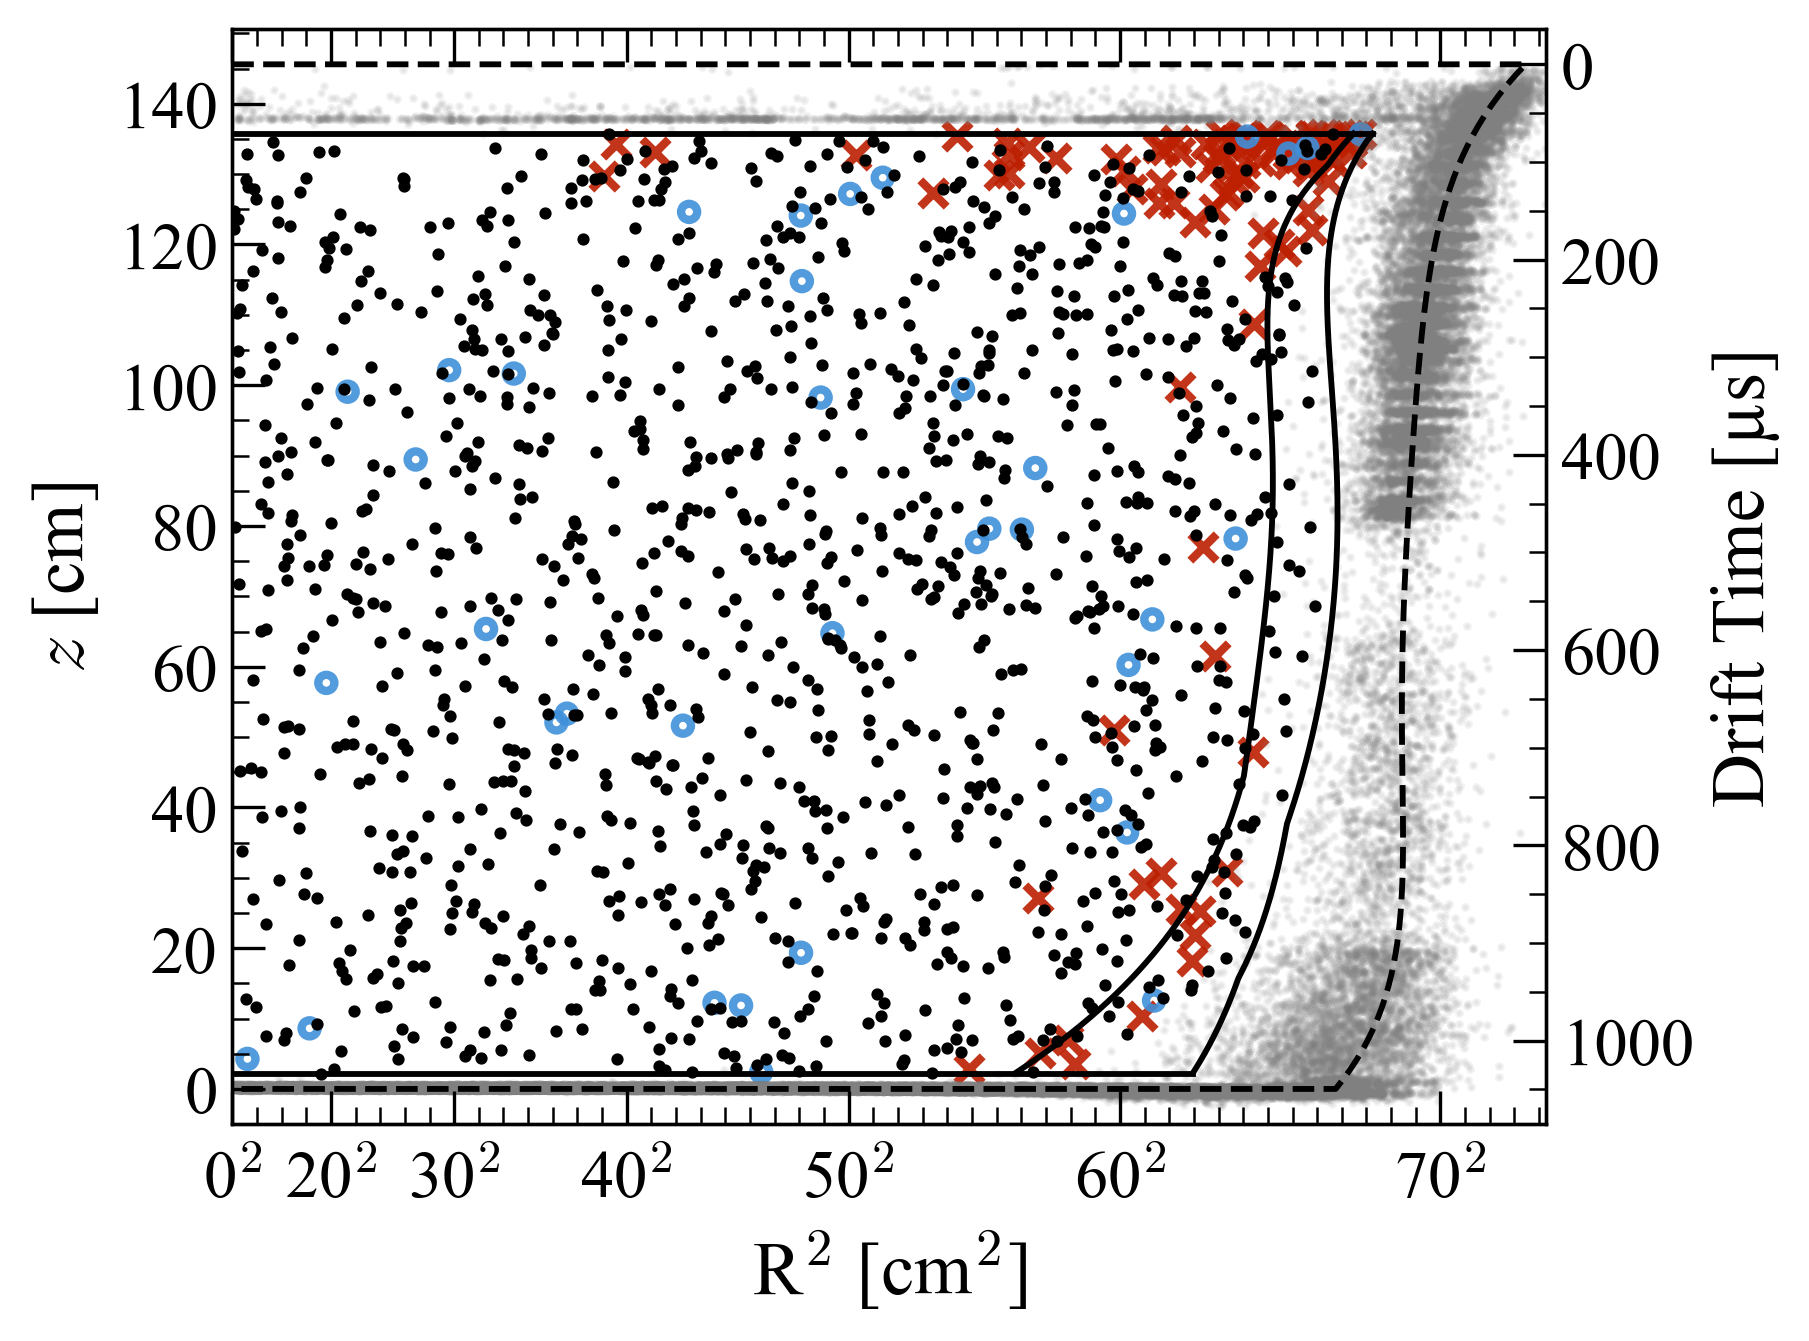
\includegraphics[width=0.85\textwidth,height=0.6\textheight,keepaspectratio]{fig-10.png}
\caption{Figure 1: Data from WS2024, in black with all analysis cuts applied, and in gray outside the FV without veto coincidence cuts. Red crosses and blue circles represent events that are vetoed by the prompt and delayed veto coincidence cuts, respectively. The dashed line shows the active volume, averaged over azimuth, and the two solid lines depict the FV, at the azimuths of its smallest and largest radial extent. The drift field affects the position reconstruction such that the observed radius of the TPC varies as a function of both drift time and azimuthal angle. [arXiv:2410.17036] Reproduced from arXiv:2410.17036 (extracted with \texttt{get\_paper\_figures}).}
\label{fig:10}
\end{figure}

\begin{figure}[H]
\centering
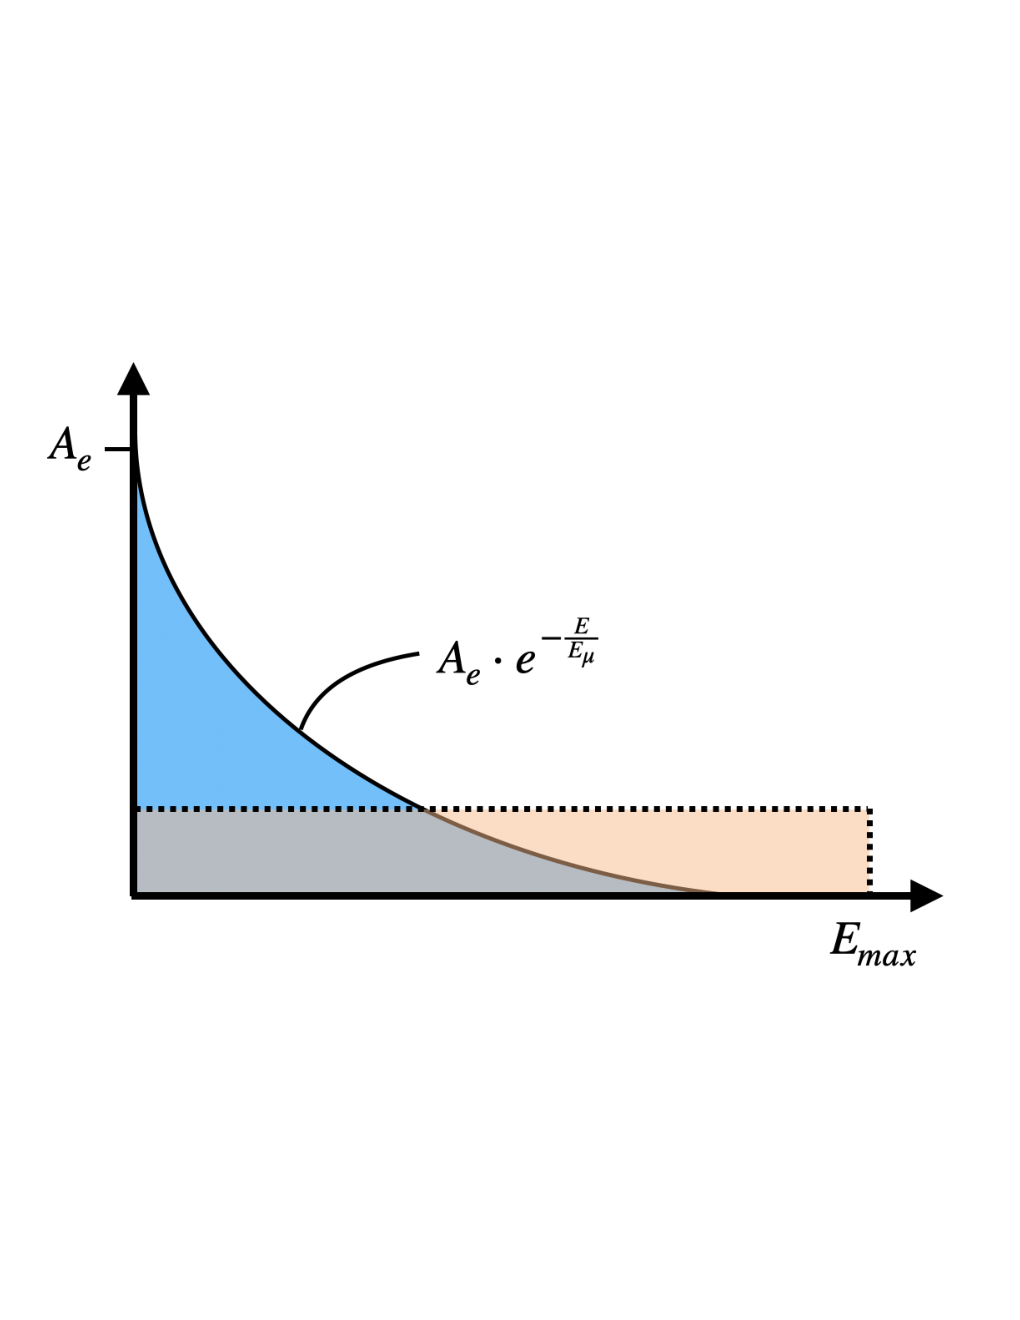
\includegraphics[width=0.85\textwidth,height=0.6\textheight,keepaspectratio]{fig-11.png}
\caption{Figure S4: Distribution from which the salt events are drawn. The parameters are described in the text. [arXiv:2410.17036] Reproduced from arXiv:2410.17036 (extracted with \texttt{get\_paper\_figures}).}
\label{fig:11}
\end{figure}

\begin{figure}[H]
\centering
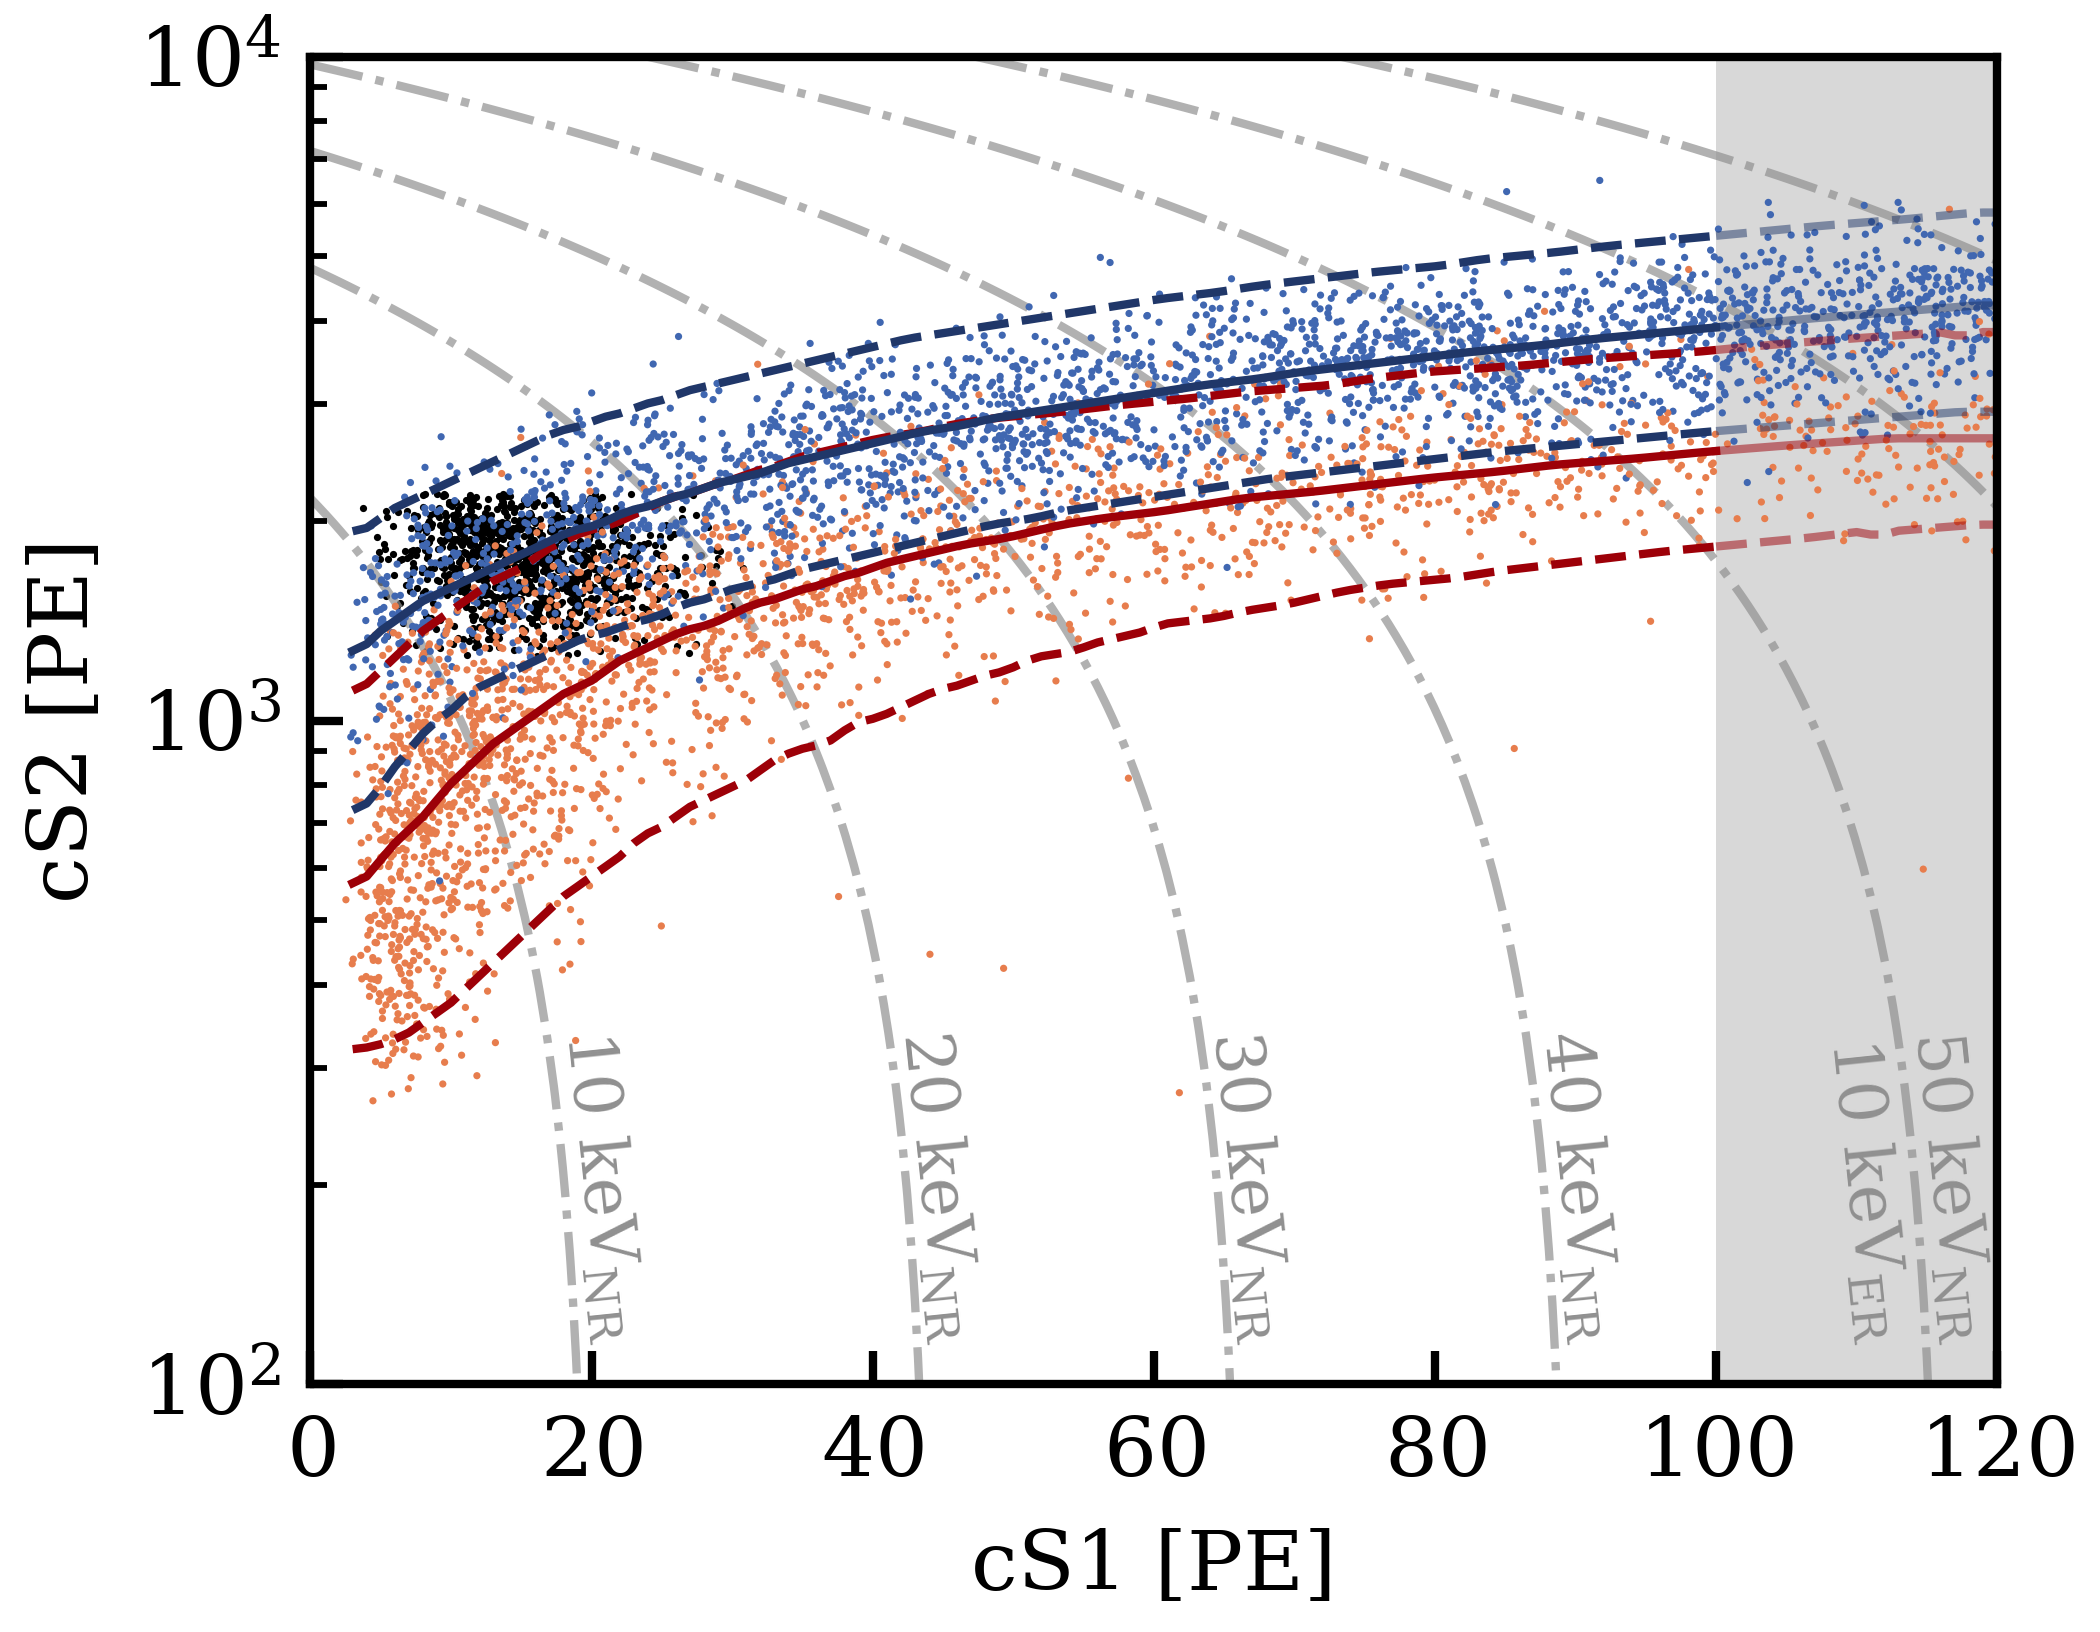
\includegraphics[width=0.85\textwidth,height=0.6\textheight,keepaspectratio]{fig-12.png}
\caption{Figure 1: NR and ER calibration data from \{\}\textasciicircum{}\{\textbackslash{}makebox[11.95839pt][r]\{\$\textbackslash{}scriptstyle 241\$\}\}\_\{\textbackslash{}makebox[11.95839pt][r]\{\$\textbackslash{}scriptstyle\$\}\}\textbackslash{}mathrm\{AmBe\} (orange), \{\}\textasciicircum{}\{\textbackslash{}makebox[11.95839pt][r]\{\$\textbackslash{}scriptstyle 220\$\}\}\_\{\textbackslash{}makebox[11.95839pt][r]\{\$\textbackslash{}scriptstyle\$\}\}\textbackslash{}mathrm\{Rn\} (blue) and \{\}\textasciicircum{}\{\textbackslash{}makebox[7.97226pt][r]\{\$\textbackslash{}scriptstyle 37\$\}\}\_\{\textbackslash{}makebox[7.97226pt][r]\{\$\textbackslash{}scriptstyle\$\}\}\textbackslash{}mathrm\{Ar\} (black). The median and the \textbackslash{}pm 2\textbackslash{}text\{\textbackslash{},\}\textbackslash{}sigma contours of the NR and ER model are shown in blue and red respectively. The gray dash-dotted contour lines show the reconstructed NR energy (\textbackslash{}mathrm\{\$\textbackslash{}mathrm\{k\}\textbackslash{}mathrm\{e\}\textbackslash{}mathrm\{V\}\$\{\} [arXiv:2303.14729] Reproduced from arXiv:2303.14729 (extracted with \texttt{get\_paper\_figures}).}
\label{fig:12}
\end{figure}

\begin{figure}[H]
\centering
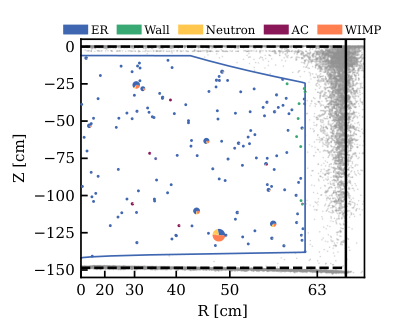
\includegraphics[width=0.85\textwidth,height=0.6\textheight,keepaspectratio]{fig-13.png}
\caption{Figure A.2: Spatial distribution of the search data in the 4.18\textbackslash{}text\{\textbackslash{},\}\textbackslash{}mathrm\{t\} fiducial volume (blue line). Each event is represented with a pie-chart, showing the fraction of the best-fit PDF including a 200\textbackslash{}text\{\textbackslash{},\}\textbackslash{}mathrm\{GeV\}\textbackslash{}text\{/\}\{\textbackslash{}mathrm\{\textbackslash{}text\{\$c\$\}\}\}\textasciicircum{}\{2\} WIMP evaluated at the position of the event, color-coded as in Figure 3. Events reconstructed outside of the fiducial volume are colored in gray. Black dashed lines depict the boundaries of the sensitive volume given by the cathode and gate positions. The TPC radius is indicated by a vertical black line. [arXiv:2303.14729] Reproduced from arXiv:2303.14729 (extracted with \texttt{get\_paper\_figures}).}
\label{fig:13}
\end{figure}

\begin{figure}[H]
\centering
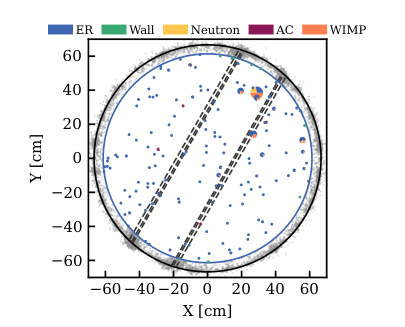
\includegraphics[width=0.85\textwidth,height=0.6\textheight,keepaspectratio]{fig-14.png}
\caption{Figure A.3: Distribution of the search data in the horizontal plane. Each event is represented with a pie-chart, showing the fraction of the best-fit PDF including a 200\textbackslash{}text\{\textbackslash{},\}\textbackslash{}mathrm\{GeV\}\textbackslash{}text\{/\}\{\textbackslash{}mathrm\{\textbackslash{}text\{\$c\$\}\}\}\textasciicircum{}\{2\} WIMP evaluated at the position of the event, color-coded as in Figure 3. Events with a reconstructed radius outside of the fiducial volume are shown in gray. The inner (outer) circle indicates the FV selection (TPC radius), and dashed lines show the transverse wire positions. [arXiv:2303.14729] Reproduced from arXiv:2303.14729 (extracted with \texttt{get\_paper\_figures}).}
\label{fig:14}
\end{figure}

\end{document}
